\documentclass[conference]{IEEEtran}
\usepackage[utf8]{inputenc}
\usepackage[T1]{fontenc}
\usepackage{amsmath,amssymb}
\usepackage{booktabs}
\usepackage{array}
\usepackage{multirow}
\usepackage{graphicx}
\usepackage{float}
\usepackage{xcolor}
\usepackage{tikz}
\usetikzlibrary{arrows.meta,positioning,calc}
\definecolor{cvRed}{HTML}{E76F51}
\definecolor{cvOrange}{HTML}{E9A23B}
\definecolor{cvGreen}{HTML}{2A9D8F}
\definecolor{cvBlue}{HTML}{457B9D}
\definecolor{cvViolet}{HTML}{8064A2}
\tikzset{cvbox/.style={rectangle,rounded corners=2pt,draw=#1!75!black,fill=#1!15,thick,align=center,font=\scriptsize,inner sep=3pt},cvarr/.style={-{Stealth[length=2mm]},thick,color=black!65}}
\usepackage{cite}
\usepackage{url}
\usepackage{balance}
\def\UrlBreaks{\do\/\do-\do\_}
\graphicspath{{figures/}}
\newcommand{\mwe}{m\,w.e.}

\begin{document}

\title{Spatially Grouped Classification of Glacier Mass-Change States across the Hindu Kush Himalaya: A Retrospective ERA5-Land Baseline}

\author{Ayush Khanal\\
Student ID: 260156, CUID: 17624354\\
MSc. Data Science and Computational Intelligence\\
Softwarica College of IT and E-commerce (Coventry University)\\
\texttt{260156@softwarica.edu.np}}

\maketitle

\begin{abstract}
Annual glacier mass change across the Hindu Kush Himalaya (HKH) is heterogeneous in space and time, yet most machine-learning (ML) studies of glacier mass balance estimate a continuous value. This paper asks how well four common classifier families separate mass gain, mass loss and near balance on a prepared HKH grid, and it does so within a planning blueprint distilled from three base studies. The modelling table holds 23,698 grid-cell--hydrological-year records (697 cells of $0.5^\circ$, April--March years 1991--2024) with 17 predictors: glacier area, year and 15 ERA5-Land variables. Classes follow fixed thresholds of $\pm0.1$~\mwe, giving 64.75\% loss, 21.00\% gain and 14.25\% near balance. Logistic Regression, an RBF Support Vector Machine, Random Forest and Gradient Boosting were compared with five-fold StratifiedGroupKFold validation on 25 K-means location clusters. Gradient Boosting led (mean fold macro-F1 0.5959; pooled out-of-fold macro-F1 0.6037, balanced accuracy 0.6297, macro ROC-AUC 0.8373), but near balance remained weak (F1 0.35, precision 0.27). The study is retrospective, reuses the same folds for tuning and reporting, and applies label thresholds smaller than the median reported uncertainty. A diagnostic also shows implausible temperature and wind anomalies in the two years that contain replaced ERA5-Land months. The results are therefore a documented baseline, not an independent generalization estimate.
\end{abstract}

\begin{IEEEkeywords}
glacier mass change, Hindu Kush Himalaya, ERA5-Land, multi-class classification, spatial cross-validation, class imbalance, computational complexity
\end{IEEEkeywords}

\section{Introduction}
Glaciers store freshwater and integrate atmospheric forcing over years to decades. Their mass balance, expressed here in metres of water equivalent (\mwe), is a key indicator of climate change. Sustained negative balance contributes to glacier retreat, changes in seasonal runoff and the growth of glacial lakes. Global assessments document accelerated glacier loss, while High Mountain Asia studies show substantial regional and temporal variability \cite{hugonnet2021,miles2021,bhattacharya2021,barandun2021}. Warming scenarios indicate further changes to glacier extent and water resources \cite{rounce2023}. Nepal-focused synthesis and long in-situ records provide additional regional context \cite{khadka2023,stumm2021}.

Observation remains difficult in the HKH. Stake measurements cover relatively few glaciers; geodetic elevation differencing is often multi-year; and physically based energy-balance models require inputs and calibration that are difficult to obtain across steep terrain. Gridded products combining glaciological and geodetic evidence provide annual mass-change targets \cite{wgmsgrid,dussaillant2024}, while ERA5-Land supplies spatially continuous climate predictors \cite{era5landpaper,era5land}. Their combination motivates a classification question: can same-year climate and glacier-area features distinguish grid-cell mass loss, gain and near balance, and how does performance change when complete spatial groups are withheld?

Classification is relevant to screening decisions but removes information about within-class magnitude. It also requires a boundary for near balance, making label uncertainty central to interpretation. The principal objective is to build and evaluate a reproducible baseline for classifying annual mass-change state across 697 HKH grid cells using 17 predictors and spatially grouped validation. Supporting analyses compare four classifier families, describe class-specific errors, examine label uncertainty and data quality, and report computational cost.

The study follows an experimental blueprint derived from three base papers \cite{gurung2025,khadka2023,anilkumar2023}. The blueprint informs the paper structure and planned safeguards, but several stronger elements—including uncertainty-defined labels, nested spatial validation and a locked temporal test—were not executed in the primary spatial experiment. Section~\ref{sec:blueprint} records these differences rather than implying that planned work was completed.

The empirical contributions are limited to: (i) documenting the prepared HKH cell-year classification table and its processing caveats; (ii) comparing linear, kernel and tree-ensemble classifiers under shared location-cluster folds; and (iii) quantifying label ambiguity and an apparent ERA5-Land discontinuity associated with replaced months \cite{ecmwfissue}. No new algorithm, causal explanation, forecast or glacier-level inference is claimed. The remainder of the paper reviews related work, audits the blueprint, describes data and methods, reports results and limitations, and concludes with future work.

\section{Related Work and Research Gap}\label{sec:related}
\subsection{Glacier change and regional evidence}
Global and regional syntheses establish widespread glacier loss and strong spatial heterogeneity. Hugonnet et al. document accelerated global elevation loss \cite{hugonnet2021}; studies of High Mountain Asia describe glacier health, rising loss rates and spatially contrasting mass-balance behaviour \cite{miles2021,bhattacharya2021,barandun2021}. Projections link additional warming to future glacier evolution and water resources \cite{rounce2023}. Nepal-focused synthesis and in-situ records provide regional context, including observations from Yala and Rikha Samba \cite{khadka2023,stumm2021}. Field and remote-sensing studies from other mountain regions add local evidence \cite{mehta2021,zhang2021}. These studies differ in spatial unit, observation basis and target definition, so they motivate but do not directly benchmark the present grid-cell classification.

\subsection{Machine learning for glacier mass balance}
Anilkumar et al. compared linear regression with nonlinear learners for point mass balance in the Alps \cite{anilkumar2023}. Gurung et al. used glacier-grouped validation for Central Himalayan mass-balance modelling and discussed radiation and monsoon predictors \cite{gurung2025}. Other studies combine ERA5-Land, geodetic targets and ensemble learning across High Mountain Asia and Central Asia \cite{ren2024,peng2025}. XGBoost performed best \cite{peng2025}. Xu et al. combined linear models, ensemble learning and OGGM to study drivers on the Tanggula Mountains \cite{xu2025}. Two recent studies address small or sparse data directly: van der Meer et al. propose a minimal ML model for very small point-balance datasets \cite{vanmeer2025}, and Sjursen et al. use XGBoost trained on sparse seasonal and annual measurements to predict mass balance on unmonitored glaciers \cite{sjursen2025}.

The literature supports nonlinear climate-based modelling but also highlights the need to test transfer beyond related observations. Grouped validation can reduce repeated-location leakage, although its interpretation is debated: spatial cross-validation is not automatically an unbiased estimate of map accuracy, for which design-based sampling has been advocated \cite{roberts2017,meyer2021,wadoux2021}. Here, grouped folds support a relative model comparison and a check against repeated-location leakage, not a map-accuracy claim.

\subsection{Comparison with the three base papers}
Table~\ref{tab:gap} compares the base studies with this work. All three treat mass balance as a numerical quantity or describe it narratively; none, as far as the blueprint review shows, defines a three-class target. The review behind this statement was limited and not systematic, so it supports a description of what the base papers do, not a claim that classification has never been attempted.

\begin{table*}[t]
\caption{Research-gap comparison between the three mandatory base papers and the present study.}
\label{tab:gap}
\centering
\footnotesize
\setlength{\tabcolsep}{3pt}
\begin{tabular}{p{0.14\textwidth}p{0.10\textwidth}p{0.16\textwidth}p{0.14\textwidth}p{0.20\textwidth}p{0.16\textwidth}}
\toprule
Previous study & Region & Data & Method & Main limitation or gap & Treatment here\\
\midrule
Gurung et al. 2025 \cite{gurung2025} & Central Himalaya (HMA regions 14--15) & ERA5-Land, topography, geodetic target 2000--2019 & Ridge, Lasso, XGBoost, MLP; glacier-grouped folds & Regression target; neighbouring glaciers can still share climate; radiation signal weak; target period fixed & Classification target; location-cluster folds; 1991--2024 annual panel\\
Khadka et al. 2023 \cite{khadka2023} & Nepal & Literature, ICIMOD inventories & Narrative review with own inventory analysis & No predictive model, no uncertainty propagation; few high-elevation stations & Quantitative baseline; reported-uncertainty diagnostic\\
Anilkumar et al. 2023 \cite{anilkumar2023} & Central Alps & ERA5-Land monthly, WGMS point data & RF, GBR, SVM, ANN vs linear; random 70/30 split & Point regression; random split with repeated sites; temperate Alps & Grid cells across HKH; same four-family design; grouped folds\\
This study & HKH, 697 cells & C3S/WGMS gridded target, ERA5-Land, glacier area & LR, SVM-RBF, RF, GB; 5-fold SGKF, 25 clusters & Retrospective; same-fold tuning; fixed thresholds; no nested CV or locked test & Disclosed and diagnosed (Sections~\ref{sec:discussion}--\ref{sec:threats})\\
\bottomrule
\end{tabular}
\end{table*}

\subsection{The research gap}
The gap is narrow and stated as scope, data and design, not as absence of prior work. What previous research has established is that nonlinear learners can exploit ERA5-Land predictors for mass balance and that validation design matters. What remains insufficiently documented is a transparent, reproducible comparison of standard classifier families on the \emph{gridded annual product} over the \emph{whole HKH footprint}, with class-wise results, explicit label-uncertainty diagnostics and a stated computational cost. This study contributes such a baseline and the diagnostics that qualify it. It does not claim novelty from using any particular algorithm, nor that classification, spatial grouping or the HKH scope is new in itself.

\section{Blueprint Audit: Planned Commitment, Executed Treatment, and Status}\label{sec:blueprint}
The blueprint is a worksheet completed for each of the three base papers. It records expected paper elements, their presence in each source study and their intended adaptation. It informed the section structure used here: introduction, literature review, context, methodology, results, discussion, limitations and conclusion.

The executed design adopts model diversity from Anilkumar et al., glacier-aware validation from Gurung et al., and context-first reporting from Khadka et al. \cite{anilkumar2023,gurung2025,khadka2023}. Spatial grouping addresses repeated-location leakage but does not create buffered geographic independence. The paper also follows the blueprint's restrained novelty language and records data limitations rather than inferring unmeasured high-elevation performance.

\begin{table*}[t]
\caption{Blueprint audit: planned commitment, executed treatment in this paper, and evidence-based status.}
\label{tab:fidelity}
\centering\footnotesize
\setlength{\tabcolsep}{3pt}
\begin{tabular}{p{0.18\textwidth}p{0.27\textwidth}p{0.34\textwidth}p{0.10\textwidth}}
\toprule
Planned commitment & Planned treatment & Executed treatment and evidence & Status\\
\midrule
Study scope & Nepal-focused grid and time series & The integration and classification notebooks retain 697 HKH cells and 23,698 cell-years; the executed scope supersedes the earlier Nepal-only plan. & Modified\\
Target construction & Uncertainty-aware three-class target & Executed target uses fixed $\pm0.1$~\mwe{} thresholds; uncertainty is analysed but does not set labels. & Modified\\
Classifier diversity & Linear, kernel and ensemble baselines & LR, RBF-SVM, RF and GB are implemented in the spatial notebook; GB extends the initial three-family plan. & Modified\\
Spatial validation & Grouped folds that keep locations together & K-means on 697 coordinates creates 25 groups; StratifiedGroupKFold assigns complete groups to five folds. Assertions report zero cluster overlap. & Implemented\\
Fold-safe preprocessing & Fit learned transformations on training data & StandardScaler is inside LR/SVM pipelines; GB sample weights are calculated from each training fold. & Implemented\\
Class imbalance & Reduce majority-class dominance & Spatial experiment uses balanced weights for LR/SVM/RF and training-fold sample weights for GB; no resampling is used in this final spatial experiment. & Implemented\\
Evaluation & Macro-F1, balanced accuracy and class-wise errors & Notebook reports fold means, pooled OOF metrics, per-class precision/recall/F1, confusion matrices and one-vs-rest ROC-AUC. & Implemented\\
Uncertainty sensitivity & Use uncertainty-aware labels or boundary tests & Target uncertainty and near-boundary ambiguity are described; alternative thresholds and exclusion tests are not executed. & Partial\\
Temporal holdout & Locked future-year test set & The spatial notebook holds out clusters, not years. A separate chronological notebook has a 2020--2024 test, but it is not the primary deployed experiment. & Partial\\
Nested evaluation & Tune in inner folds and report outer folds & Hyperparameter selection and pooled OOF reporting reuse the same five spatial folds. & Open\\
Buffered spatial separation & Exclude nearby training cells around validation blocks & Cluster identity is separated, but no distance buffer or autocorrelation-based block width is implemented. & Open\\
Feature interpretation & Explain predictor contributions & Correlations and class-wise distributions are reported; the spatial notebook does not perform a supported feature-importance analysis for the primary paper. & Partial\\
Cost and memory & Repeated timings and memory profiling & Single-run fit/search timings and model size are logged; memory profiling and repeated controlled runs are absent. & Partial\\
Ablations and additional covariates & Test feature groups, topography and other covariates & The primary model retains 17 predictors; the listed ablations and topographic additions are not executed. & Open\\
\bottomrule
\end{tabular}
\end{table*}

\section{Study Area and Data Sources}\label{sec:data}
\subsection{Study area}
The prepared target grid spans $27.25^\circ$--$39.25^\circ$\,N and $67.25^\circ$--$103.75^\circ$\,E and contains 697 cells of $0.5^\circ$, each present in all 34 hydrological years (Fig.~\ref{fig:map}). This footprint covers the Hindu Kush, Karakoram, the Himalayan arc, parts of the Tibetan Plateau margin, Tien Shan and eastern ranges. The shaded envelope in Fig.~\ref{fig:map} is a smoothed outline of the occupied cells. It is not an official regional boundary, and no polygon of the HKH was used in the analysis. The original file name contains ``nepal'' for historical reasons, but the coordinates clearly extend far beyond Nepal, so the study is HKH-wide in the sense of this footprint.

\begin{figure*}[t]
\centering
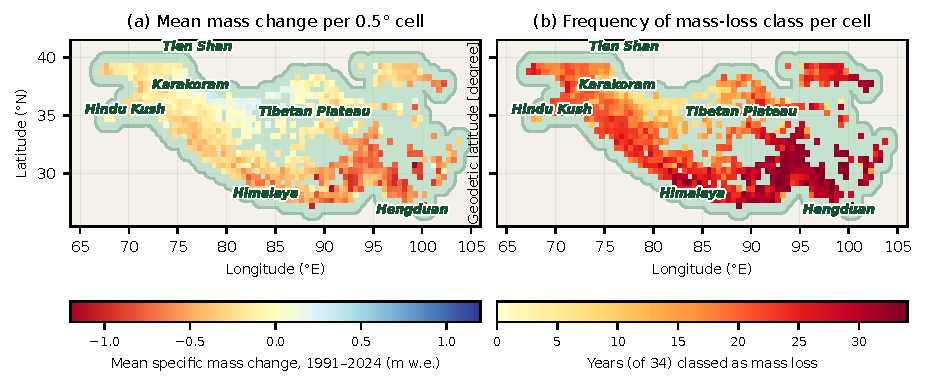
\includegraphics[width=\textwidth]{fig_study_area_map.pdf}
\caption{Study area. (a) Mean specific mass change per $0.5^\circ$ target cell, 1991--2024. (b) Number of hydrological years (of 34) in which each cell is classed as mass loss. Cells are drawn as $0.5^\circ$ squares over Natural Earth country outlines; the green shaded envelope is a smoothed outline of the 697 occupied cells and is not an official HKH boundary.}
\label{fig:map}
\end{figure*}

\subsection{Datasets}
Table~\ref{tab:datasets} lists the datasets used. The target is the Copernicus Climate Change Service (C3S) global gridded annual glacier mass-change product derived from the World Glacier Monitoring Service (WGMS) Fluctuations of Glaciers database \cite{wgmsgrid,dussaillant2024}. It distributes annual mass change and its uncertainty on a $0.5^\circ$ global grid for every hydrological year since 1975/76, assigns a glacier to the cell that contains its centroid, and warns that the annual product cannot resolve the different Northern and Southern Hemisphere hydrological-year definitions. In the prepared table the specific value in \mwe{} equals the total mass change in gigatonnes divided by water density and the glacier area carried in the same record; I verified this relation on all 23,698 rows to within rounding of the stored three-decimal values. The glacier-area column is therefore the glacierised area associated with the cell, not the cell area.

\begin{table*}[t]
\caption{Datasets, roles and sources. Resolutions are those stated in the cited documentation or observed in the prepared files.}
\label{tab:datasets}
\centering
\footnotesize
\setlength{\tabcolsep}{3pt}
\begin{tabular}{p{0.13\textwidth}p{0.11\textwidth}p{0.17\textwidth}p{0.10\textwidth}p{0.10\textwidth}p{0.12\textwidth}p{0.17\textwidth}}
\toprule
Dataset & Provider & Variables used & Spatial res. & Temporal res. & Period used & Role; access\\
\midrule
Global gridded annual glacier mass change & C3S; WGMS & Mass change (Gt, \mwe), glacier area (km$^2$), uncertainty & $0.5^\circ$ & Annual, hydrological year & 1991--2024 & Target and glacier area; DOI 10.24381/cds.ba597449 \cite{wgmsgrid}\\
ERA5-Land & ECMWF / C3S & 15 land-surface variables (Table~\ref{tab:vars}) & $0.1^\circ$(inferred grid step) & Monthly means & Apr 1990 -- Mar 2024 & Predictors; DOI 10.24381/cds.e2161bac \cite{era5land,era5landpaper}\\
ERA5-Land recovery product & ECMWF / C3S & 12 variables, Sep 2022--Feb 2024 & $0.1^\circ$ & Monthly, hour-of-day product & Sep 2022 -- Feb 2024 & Replacement for affected months \cite{ecmwfissue}\\\\
Static glacier area & Inside target product & \texttt{glacier\_area\_km2} & $0.5^\circ$ & Per record & 1991--2024 & Predictor \cite{wgmsgrid}\\
\bottomrule
\end{tabular}
\end{table*}

ERA5-Land is a land-surface reanalysis produced by replaying the land component of the ECMWF ERA5 system with atmospheric forcing, including a lapse-rate correction for the altitude difference between forcing and land grids \cite{era5land,era5landpaper}. Observations influence it only indirectly through that forcing, and the data-set documentation cautions that uncertainty grows backward in time. The inferred $0.1^\circ$ spacing in the processing notebook agrees with the documented native resolution of about 9~km, which is coarse for steep glacierised terrain and is a limitation discussed later.

Two inputs listed in an earlier plan are not used. Static grids of glacier mask and geopotential and the ICIMOD glacier inventories belong to the Nepal-oriented blueprint, and the final HKH table contains no elevation, aspect or debris-cover information. The only glacier descriptor is glacier area.

\section{Data Processing and Feature Engineering}\label{sec:processing}
\subsection{Hydrological-year convention}
The target label $Y$ denotes the hydrological year from 1 April of $Y-1$ through 31 March of $Y$, a half-open interval $[\text{1 April } Y{-}1,\ \text{1 April } Y)$. The C3S documentation gives April to March as the Northern Hemisphere convention \cite{wgmsgrid}. The annual table stores a \texttt{time} stamp of 1 January of the label year, which is a label and not the start of the period. Every one of the 23,698 cell-year groups has all 12 distinct months, so no incomplete year occurs and none was imputed. Month $m$ and calendar year $c$ map to the label
\begin{equation}
Y(c,m)=c+\mathbb{1}[m\ge 4],
\label{eq:hy}
\end{equation}
where $\mathbb{1}[\cdot]$ is the indicator function.

\subsection{Spatial alignment of ERA5-Land with the target grid}
Each $0.5^\circ$ target cell is matched to the $0.1^\circ$ ERA5-Land cells that overlap it by conservative area-weighted averaging. The weight of a source cell is proportional to $\Delta\lambda(\sin\varphi_N-\sin\varphi_S)$ for its overlap rectangle, which is the spherical area factor, and the common radius term cancels. A target cell is retained when at least 70\% of its area is covered; the minimum observed coverage was 0.7007, the mean 0.9888, and the median and upper quartile were 1.0. The lowest-coverage cells lie on the northern edge near $39.25^\circ$\,N. All 697 target cells passed, and the monthly regridded table has 284,376 rows, that is 408 months times 697 cells, with no duplicate keys and no missing month. The workflow therefore does not interpolate across target cells; it averages source cells that geometrically overlap each target cell. Coordinates in the table are the target-cell centres.

\subsection{Predictors and aggregation rules}
The 17 predictors are glacier area, hydrological year and 15 ERA5-Land variables (Table~\ref{tab:vars}). Coordinates, the continuous target, its uncertainty, the gigatonne columns and integration metadata are excluded. No feature selection and no dimensionality reduction were applied. Aggregation to the hydrological year is variable specific, because accumulated, instantaneous and state variables need different treatment. State variables and winds are day-weighted means of the monthly values. The monthly-mean-of-daily-mean (``moda'') product expresses accumulated variables as a per-day quantity, so water-flux variables are summed over months after multiplying by the days in each month, and radiation, given as daily accumulated energy, is converted to a mean flux. These are the rules implemented in the integration notebook and documented in its metadata table; the metadata audit still flags all 15 variables for review against the original NetCDF attributes, and I treat the rules as implemented but not independently certified.

\begin{table*}[t]
\caption{Predictors, physical meaning, source units and annual operation as implemented in the integration notebook. Values in the last column are table means over all 23,698 records.}
\label{tab:vars}
\centering
\footnotesize
\setlength{\tabcolsep}{3pt}
\begin{tabular}{llp{0.20\textwidth}p{0.18\textwidth}p{0.20\textwidth}r}
\toprule
Name & Group & Meaning & Source unit & Annual operation & Mean\\
\midrule
\texttt{glacier\_area\_km2} & Glacier & Associated glacierised area & km$^2$ & Carried from target & 114.08\\
\texttt{hydrological\_year} & Time & Year label $Y$ & year & Label & --\\
\texttt{t2m} & Ablation & 2-m air temperature & K & Day-weighted mean & 268.5\\
\texttt{snowc} & Accumulation & Snow cover & fraction; exported scale 0--100 & Day-weighted mean & 41.7\\
\texttt{sde} & Accumulation & Snow depth & m & Day-weighted mean & 1.24\\
\texttt{sd} & Accumulation & Snow water equivalent depth & m w.e. & Day-weighted mean & 0.362\\
\texttt{sf} & Accumulation & Snowfall & m w.e. per day & Sum of daily-mean accumulations & 0.366\\
\texttt{smlt} & Ablation & Snowmelt & m w.e. per day & Sum of daily-mean accumulations & 0.330\\
\texttt{ssr} & Energy & Net surface solar radiation & J\,m$^{-2}$ per day & Mean daily energy as flux & 138.2\\
\texttt{str} & Energy & Net surface thermal radiation & J\,m$^{-2}$ per day & Mean daily energy as flux & $-$79.8\\
\texttt{ro} & Water flux & Total runoff & m per day & Sum of daily-mean accumulations & 0.504\\
\texttt{es} & Water flux & Snow evaporation & m w.e. per day & Sum of daily-mean accumulations & $-$0.035\\
\texttt{sro} & Water flux & Surface runoff & m per day & Sum of daily-mean accumulations & 0.268\\
\texttt{e} & Water flux & Total evaporation & m w.e. per day & Sum of daily-mean accumulations & $-$0.359\\
\texttt{u10}, \texttt{v10} & Wind & 10-m wind components & m\,s$^{-1}$ & Day-weighted mean & 0.54, 0.38\\
\texttt{tp} & Accumulation & Total precipitation & m per day & Sum of daily-mean accumulations & 0.874\\
\bottomrule
\end{tabular}
\end{table*}

The predictor groups represent temperature and melt, snow and snowfall, radiation, runoff, evaporation and wind. They motivate the climate feature set but do not make the classifier a surface-energy-balance model. The notebook's aggregation rules are implemented; original NetCDF unit and metadata certification remains open.

\subsection{The September 2022--February 2024 ERA5-Land issue}\label{sec:issue}
ECMWF reported an issue in ERA5-Land monthly averaged reanalysis for September 2022--February 2024, affecting accumulated variables globally \cite{ecmwfissue}. The recommended recovery uses the monthly averaged reanalysis by hour of day at 00:00; corrected monthly data are available from March 2024. The affected accumulations therefore required explicit handling before annual aggregation.

The integration notebook replaces 12 variables (\texttt{t2m, sf, smlt, ssr, str, ro, es, sro, e, u10, v10, tp}) across the 18 affected months by joining a recovery table on year-month and source coordinates. Its audit reports complete replacement coverage and no missing values after the join. Three variables (\texttt{snowc}, \texttt{sde}, \texttt{sd}) remain from the original source. Seven affected months fall in HY2023 and eleven in HY2024; no rows were dropped, and the modelling table retains all 23,698 records.

The join does not establish scientific equivalence. The accumulation period represented by the 00:00 recovery product was not independently verified, and \texttt{t2m}, \texttt{u10} and \texttt{v10} are not accumulated variables, so replacing their monthly means with hour-specific values is not justified by the ECMWF notice. Section~\ref{sec:diag} shows anomalies coincident with the replacement. The issue is therefore handled by replacement with unresolved semantics, not certified as corrected.

\subsection{Resulting modelling table}
The final table contains 23,698 rows, 697 locations and 34 years, with no duplicate year-location keys or missing retained predictors. Mass change has mean $-0.2966$~\mwe, median $-0.2775$~\mwe and range $[-2.143,1.181]$~\mwe; 72.3\% of values are negative. Collinearity is strong: $r$ is approximately 1.00 for \texttt{sde}/\texttt{sd}, 0.98 for \texttt{ro}/\texttt{tp}, 0.97 for \texttt{ro}/\texttt{sro}, and $-0.93$ for \texttt{snowc}/\texttt{ssr}. These pooled correlations mix spatial and temporal variation.

\begin{figure*}[t]
\centering
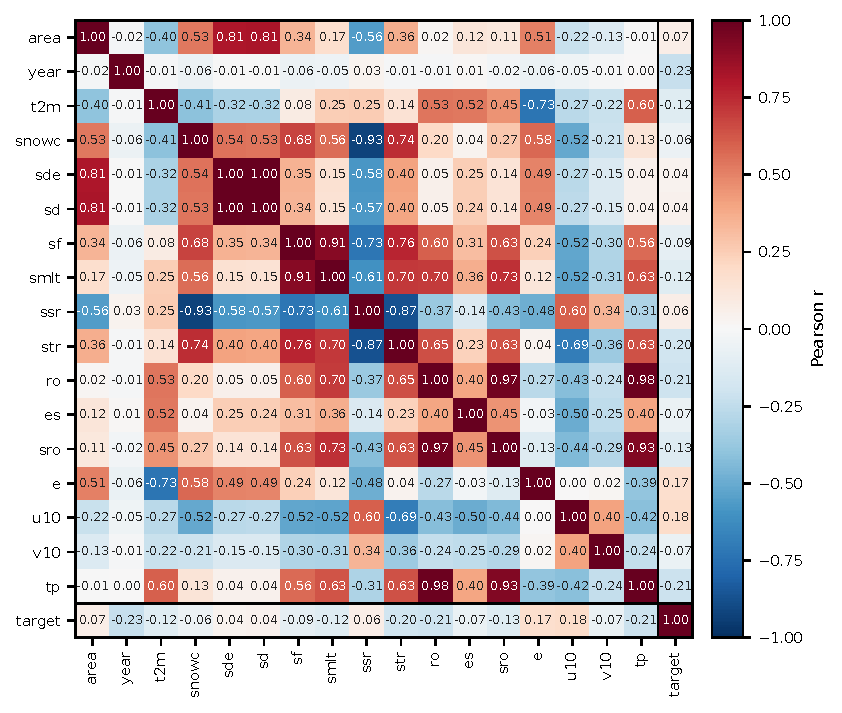
\includegraphics[width=\textwidth]{fig_correlation.pdf}
\caption{Pearson correlation among the 17 predictors and the continuous target (last row and column), pooled over all records. Each cell is annotated with the signed Pearson coefficient $r$ (two decimals); larger $|r|$ indicates stronger linear association. Collinearity is high within the snow, runoff and radiation groups.}
\label{fig:corr}
\end{figure*}

\section{Problem Formulation}\label{sec:problem}
Let $i=1,\dots,N$ index records, with $N=23{,}698$, each defined by a location $\ell_i\in\{1,\dots,L\}$, $L=697$, and a hydrological year $Y_i\in\{1991,\dots,2024\}$. Let $m_i$ be the specific mass change in \mwe{} and $u_i$ its reported uncertainty. The feature vector is $\mathbf{x}_i\in\mathbb{R}^{p}$ with $p=17$. The three-class label is
\begin{equation}
y_i=
\begin{cases}
\text{gain}, & m_i>\tau,\\
\text{loss}, & m_i<-\tau,\\
\text{near balance}, & -\tau\le m_i\le\tau,
\end{cases}
\qquad \tau=0.1~\mwe.
\label{eq:classes}
\end{equation}
The learning problem is to estimate a classifier $f:\mathbb{R}^{p}\to\{1,2,3\}$ that minimises expected misclassification across classes under a validation scheme that holds out whole spatial groups. With $K=3$ classes and training set $\mathcal{D}_{\text{tr}}$ of size $n$, empirical risk minimisation with class weights $w_k$ gives
\begin{equation}
\hat f=\arg\min_{f\in\mathcal{F}}\ \frac{1}{n}\sum_{i\in\mathcal{D}_{\text{tr}}} w_{y_i}\,\mathcal{L}\!\left(y_i,f(\mathbf{x}_i)\right)+\Omega(f),
\label{eq:erm}
\end{equation}
where $\mathcal{L}$ is the model-specific loss and $\Omega$ a regulariser.

The task is retrospective: $\mathbf{x}_i$ summarises the same hydrological year as the label, so the classifier cannot be applied before the year ends. The folds hold out locations and not years, so the experiment tests transfer to unseen \emph{places} within the observed period and does not test forecasting. The threshold $\tau$ is a project convention and is not adjusted to the product's uncertainty, which has mean 0.2635~\mwe{} and median 0.186~\mwe{}. Converting a continuous quantity to three bins also discards magnitude, and rows near $\pm\tau$ can flip class under small changes in the target.

\section{Methodology}\label{sec:method}
The executed pipeline is summarised in Fig.~\ref{fig:methodflow}. It starts from the C3S/WGMS gridded mass-change target and ERA5-Land monthly climate fields, applies the documented preprocessing and spatial/temporal alignment, constructs the 17-feature table, evaluates four classifiers under grouped spatial folds, and saves the selected spatial Gradient Boosting estimator for the Streamlit application. The separate chronological imbalance experiment is not part of the deployed pipeline.

\begin{figure*}[t]
\centering
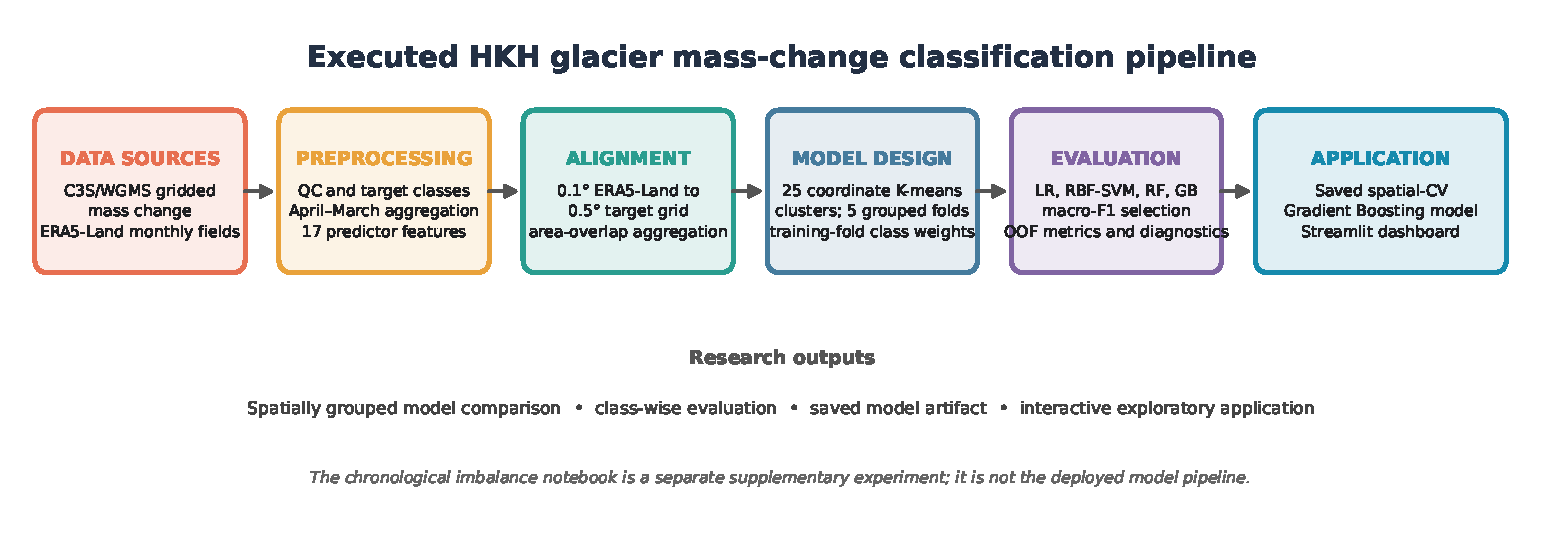
\includegraphics[width=\textwidth]{fig_method_workflow.pdf}
\caption{Executed project workflow from source products to the Streamlit application. The figure includes only stages documented in the supplied notebooks, README and application source.}
\label{fig:methodflow}
\end{figure*}
\subsection{Classifiers}
Four classifiers were fitted in scikit-learn using the same 17 predictors and the same five spatial folds. The comparison was designed to test a linear baseline, a nonlinear kernel classifier, a bagged tree ensemble and a boosted tree ensemble. The notebook searches 21 configurations in total (3 LR, 2 SVM, 8 RF and 8 GB), giving 105 training-fold fits. Each candidate is ranked by mean validation macro-F1, with balanced accuracy and accuracy used as tie-breakers.

\emph{Logistic Regression (LR)} is the linear reference. Its pipeline applies \texttt{StandardScaler} before multinomial logistic regression, with \texttt{class\_weight=balanced}, \texttt{max\_iter=2000} and seed 42. The search varies $C\in\{0.1,1,10\}$; the selected setting is $C=10$. Scaling is fitted separately within each training fold. LR is computationally inexpensive and provides a useful low-capacity comparator, but its pooled OOF macro-F1 is 0.4180 and it has the weakest near-balance F1 (0.20).

\emph{RBF Support Vector Machine (SVM)} provides a nonlinear margin-based comparison. It uses a StandardScaler--SVC pipeline, balanced class weights, $C\in\{1,5\}$, \texttt{gamma=scale}, one-vs-rest decision scores and \texttt{probability=False}. The selected setting is $C=5$. The notebook uses decision scores for ROC analysis rather than fitting probability calibration. Its pooled OOF macro-F1 is 0.4471; it improves on LR but remains below both tree ensembles \cite{cortes1995}.

\emph{Random Forest (RF)} tests bagged decision trees without feature scaling. It uses \texttt{class\_weight=balanced\_subsample}, parallel workers and seed 42. The grid varies tree count (150 or 300), maximum depth (12 or unrestricted) and minimum leaf size (1 or 3). The selected configuration has 300 trees, depth 12 and minimum leaf size 3. Its pooled OOF macro-F1 is 0.5294 \cite{breiman2001}. The training--validation gap and the unrestricted-depth candidates show why depth and leaf-size controls matter in this dataset.

\emph{Gradient Boosting (GB)} is the selected model. The search varies 100/200 estimators, learning rate 0.05/0.1 and maximum depth 2/3. The winning configuration uses 200 estimators, learning rate 0.1 and depth 3. Since \texttt{GradientBoostingClassifier} does not expose a class-weight parameter, the notebook computes balanced per-record sample weights from each training fold and passes them to \texttt{fit}. The pooled OOF macro-F1 is 0.6037, the highest of the four \cite{friedman2001}; however, near-balance F1 is only 0.35. The saved model is fitted on all 23,698 records for application use, and that final fit is not a separate evaluation.

All four models are evaluated on the identical held-out spatial clusters in each fold. The notebook records accuracy, balanced accuracy and macro-F1 during tuning, then creates pooled out-of-fold predictions for class-wise precision, recall, F1, confusion matrices and one-vs-rest ROC-AUC. Because the same folds select and report the models, these values are comparative spatial-CV diagnostics rather than an unbiased independent test estimate.

\subsection{Preprocessing and class-imbalance handling}
LR and SVM sit in pipelines with a standard scaler,
\begin{equation}
\tilde x_{j}=\frac{x_{j}-\mu_{j}^{\text{tr}}}{\sigma_{j}^{\text{tr}}},
\label{eq:scale}
\end{equation}
whose mean $\mu_j^{\text{tr}}$ and standard deviation $\sigma_j^{\text{tr}}$ are estimated on the training portion of each fold only. Tree models need no scaling.

Class imbalance is handled by cost-sensitive weighting; no resampling is used. The balanced weight of class $k$ computed on a training set of size $n$ is
\begin{equation}
w_k=\frac{n}{K\,n_k},
\label{eq:cw}
\end{equation}
where $n_k$ is the number of training records of class $k$. LR and SVM use the library's \texttt{balanced} option, RF uses \texttt{balanced\_subsample}, which recomputes weights within each bootstrap sample, and GB receives per-record sample weights computed from the labels of the current training fold. Weights are therefore derived from training data only, and the validation partition is never weighted or resampled. Random undersampling and combined schemes were not part of the final experiment, and a no-weighting control was not run, so the paper cannot say how much weighting helps relative to doing nothing.

\subsection{Spatially grouped validation}
The 697 unique coordinate pairs were standardised by axis and clustered by $k$-means \cite{lloyd1982} with $k=25$, 20 initialisations and seed 42. The objective is
\begin{equation}
\min_{\{C_c\}}\sum_{c=1}^{25}\sum_{\ell\in C_c}\left\|\mathbf{z}_\ell-\boldsymbol{\mu}_c\right\|_2^2,
\label{eq:kmeans}
\end{equation}
where $\mathbf{z}_\ell$ are the standardised coordinates and $\boldsymbol{\mu}_c$ the cluster centroid. Each location's 34 records inherit one cluster label. Cluster sizes range from 9 to 40 locations (mean 27.9, median 29). Five-fold StratifiedGroupKFold with shuffling and seed 42 then assigns whole clusters to folds while trying to preserve class proportions \cite{pedregosa2011}. A built-in assertion verifies that no cluster is shared between training and validation in any fold, and it passed for all five folds. Fig.~\ref{fig:clusters} shows the clusters. Table~\ref{tab:folds} lists fold sizes and class counts.

\begin{figure*}[t]
\centering
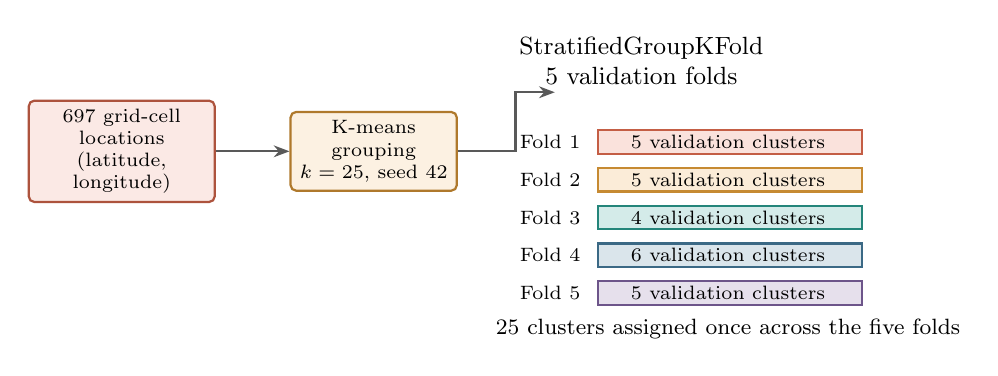
\begin{tikzpicture}[x=1cm,y=1cm]
\node[cvbox=cvRed,text width=2.15cm,minimum height=1.0cm] (loc) at (1.5,0.2) {697 grid-cell locations\\(latitude, longitude)};
\node[cvbox=cvOrange,text width=1.9cm,minimum height=1.0cm] (km) at (4.7,0.2) {K-means grouping\\$k=25$, seed 42};
\draw[cvarr] (loc.east) -- (km.west);
\node[font=\small,align=center] at (8.1,1.35) {StratifiedGroupKFold\\5 validation folds};
\draw[cvarr] (km.east) -- (6.5,0.2) -- (6.5,0.95) -- (7.0,0.95);
\foreach \i/\col/\nval in {1/cvRed/5,2/cvOrange/5,3/cvGreen/4,4/cvBlue/6,5/cvViolet/5}{
  \pgfmathsetmacro{\yy}{0.65-0.48*\i}
  \node[font=\scriptsize,anchor=east] at (7.45,\yy+0.15) {Fold \i};
  \fill[\col!20] (7.55,\yy) rectangle (10.9,\yy+0.30);
  \draw[\col!85!black,thick] (7.55,\yy) rectangle (10.9,\yy+0.30);
  \node[font=\scriptsize,align=center] at (9.2,\yy+0.15) {\nval\ validation clusters};
}
\node[font=\footnotesize,align=center] at (9.2,-2.05) {25 clusters assigned once across the five folds};
\end{tikzpicture}

\caption{Spatial cross-validation design reproduced from the executed notebook: the 697 coordinate locations are grouped into 25 K-means clusters, and complete clusters are assigned to five validation folds. The folds contain 5, 5, 4, 6 and 5 validation clusters, respectively. This is cluster-based separation, not a geographic buffer.}
\label{fig:spatialcv}
\end{figure*}

\begin{figure}[t]
\centering
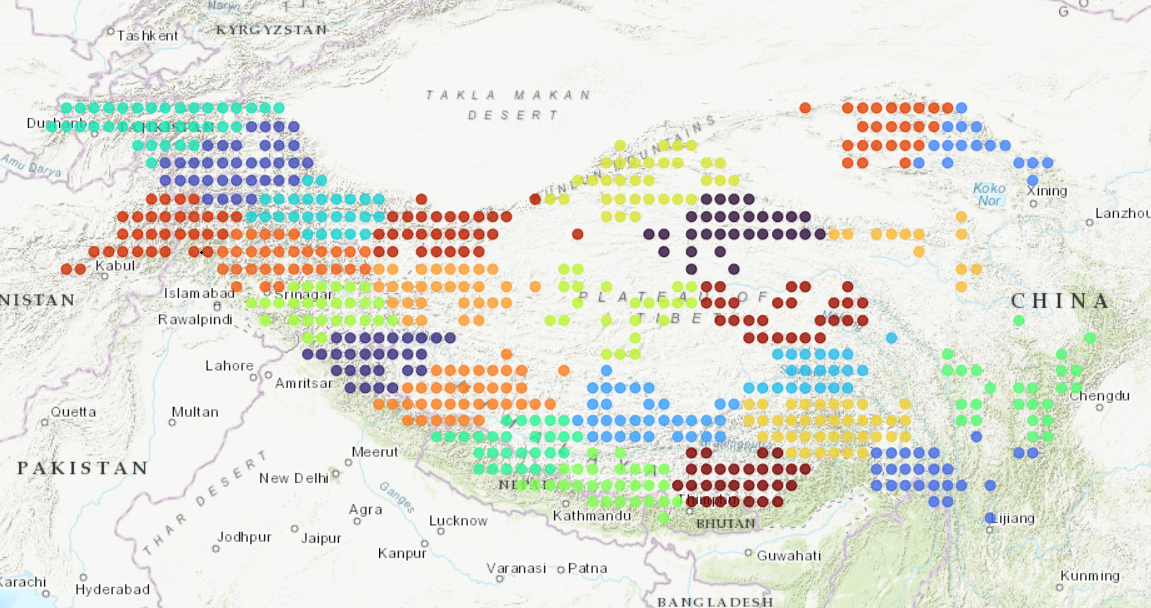
\includegraphics[width=\columnwidth]{spatial_clusters_nb.png}
\caption{K-means groups of the 697 grid locations (25 clusters, standardised coordinates). The colour map repeats across clusters, so adjacent clusters can share a colour. Groups prevent a location or cluster from crossing a fold; they are not buffered geographic blocks.}
\label{fig:clusters}
\end{figure}

\begin{table}[t]
\caption{Spatial fold composition (from the validation notebook).}
\label{tab:folds}
\centering
\scriptsize
\setlength{\tabcolsep}{1.8pt}
\begin{tabular}{crrcrrrc}
\toprule
Fold & Train & Val. & Clusters tr/val & Gain & Loss & Near & Shared\\
\midrule
1 & 19,754 & 3,944 & 20 / 5 & 863 & 2,506 & 575 & 0\\
2 & 18,904 & 4,794 & 20 / 5 & 1,111 & 3,022 & 661 & 0\\
3 & 19,924 & 3,774 & 21 / 4 & 303 & 3,111 & 360 & 0\\
4 & 18,122 & 5,576 & 19 / 6 & 1,453 & 3,192 & 931 & 0\\
5 & 18,088 & 5,610 & 20 / 5 & 1,246 & 3,513 & 851 & 0\\
\bottomrule
\end{tabular}
\end{table}

Cluster identity is separated, but geographic distance is not: adjacent cells can fall in different groups, and standardised latitude/longitude is not projected-distance clustering. A buffer based on target autocorrelation would be stronger; that range was not estimated. Fold composition also varies, from 303 validation gain records in fold 3 to 1,453 in fold 4.

\subsection{Computational complexity}
Table~\ref{tab:complexity} gives approximate theoretical costs for every algorithm in the final workflow. The expressions are order-of-magnitude and rest on stated assumptions; they are not measured times and ignore implementation constants, parallelism and caching. Here $n$ is the number of training records, $p$ the number of features, $K$ the number of classes, $I$ solver iterations, $T$ boosting iterations, $B$ trees in a forest, $\tilde p$ the number of candidate features per split ($\tilde p=\lceil\sqrt p\,\rceil$ for the classifier default), $d$ maximum tree depth, $m$ the number of support vectors, $k$ clusters and $q$ the coordinate dimension.

\begin{table*}[t]
\caption{Theoretical computational complexity of the algorithms in the final methodology, with symbols defined in the text. Assumptions: dense data, no parallelism, tree split search by sorting, and pairwise SVM decomposition.}
\label{tab:complexity}
\centering
\footnotesize
\setlength{\tabcolsep}{3pt}
\begin{tabular}{p{0.13\textwidth}p{0.20\textwidth}p{0.14\textwidth}p{0.17\textwidth}p{0.27\textwidth}}
\toprule
Algorithm & Training time & Prediction time (per sample) & Space & Main influencing parameters\\
\midrule
Logistic Regression (L-BFGS, multinomial) & $O(I\,n\,p\,K)$ & $O(pK)$ & $O(np+pK)$ & Solver iterations $I$ (cap 2000), $C$, $K$, $p$\\\\
SVM, RBF kernel (SMO, pairwise) & Between $O(n^{2}p)$ and $O(n^{3}p)$ & $O(m\,p)$ & $O(np)$ data; up to $O(n^{2})$ if the kernel matrix is cached; model $O(mp)$ & $C$, $\gamma$, class weights; $m$ grows with overlap and noise\\\\
Random Forest & $O\!\left(B\,\tilde p\,n\log n\right)$ for fully grown trees; $O(B\,\tilde p\,n\,d)$ if depth capped & $O(B\,d)$ & $O(B\,L_{\max})$ nodes with $L_{\max}\le n/s_{\min}$ for min. leaf size $s_{\min}$ & Trees $B$, depth $d$, leaf size, features per split\\\\
Gradient Boosting (depth-limited trees) & $O\!\left(T\,K\,d\,p\,n\right)$ with presorting-style split search & $O(T\,K\,d)$ & $O(T\,K\,2^{d})$ & Iterations $T$, depth $d$, learning rate $\eta$ (trade-off with $T$), $K$\\\\
$k$-means (Lloyd, spatial grouping) & $O(I\,n_{\text{loc}}\,k\,q)$ per initialisation, times 20 initialisations & $O(kq)$ to assign a point & $O(n_{\text{loc}}q+kq)$ & Clusters $k=25$, iterations $I$, locations $n_{\text{loc}}=697$, $q=2$\\\\
Standard scaler (LR, SVM) & $O(np)$ & $O(p)$ & $O(p)$ & Features $p$\\
\bottomrule
\end{tabular}
\end{table*}

These are asymptotic approximations: SVM cost depends on solver and support vectors, while tree costs depend on split-search implementation and tree shape \cite{chang2011}. The 21 candidates across five folds require 105 fits, so search cost scales with the number of configurations. At the selected settings ($n\approx19{,}000$, $p=17$, $K=3$), SVM has the steepest theoretical training growth; GB uses $T=200$, $d=3$, and RF uses $B=300$. These expressions do not predict measured wall-clock time.

\subsection{Evaluation metrics}
Let $TP_k$, $FP_k$ and $FN_k$ be the true positives, false positives and false negatives for class $k$ in the confusion matrix $\mathbf{M}$, whose entry $M_{ab}$ counts records of true class $a$ predicted as class $b$. The metrics are
\begin{align}
\mathrm{Acc}&=\frac{\sum_k TP_k}{N},\quad
P_k=\frac{TP_k}{TP_k+FP_k},\label{eq:prf}\\
R_k&=\frac{TP_k}{TP_k+FN_k},\quad
F1_k=\frac{2P_kR_k}{P_k+R_k},\label{eq:f1}\\
\mathrm{BA}&=\frac{1}{K}\sum_{k=1}^{K}R_k,\quad
\mathrm{MacroF1}=\frac{1}{K}\sum_{k=1}^{K}F1_k.\label{eq:macro}
\end{align}
One-vs-rest ROC-AUC uses each class score against the remaining classes and is macro-averaged. Macro-F1 is the selection metric because it weights classes equally; balanced accuracy and accuracy break ties \cite{sokolova2009}. Pooled OOF predictions give one held-out-cluster prediction per record.

\section{Experimental Design}\label{sec:design}
\subsection{Target distribution}
Loss accounts for 64.75\% of records, so an all-loss classifier reaches 0.6475 accuracy while missing both minority classes. This majority-class baseline is used to interpret accuracy.

\begin{table}[t]
\caption{Target-class distribution under Eq.~\eqref{eq:classes}.}
\label{tab:classes}
\centering
\footnotesize
\begin{tabular}{lrr}
\toprule
Class & Records & Share (\%)\\
\midrule
Mass loss ($m<-0.1$) & 15,344 & 64.75\\
Mass gain ($m>0.1$) & 4,976 & 21.00\\
Near balance & 3,378 & 14.25\\
\midrule
Total & 23,698 & 100.00\\
\bottomrule
\end{tabular}
\end{table}

\begin{figure*}[t]
\centering
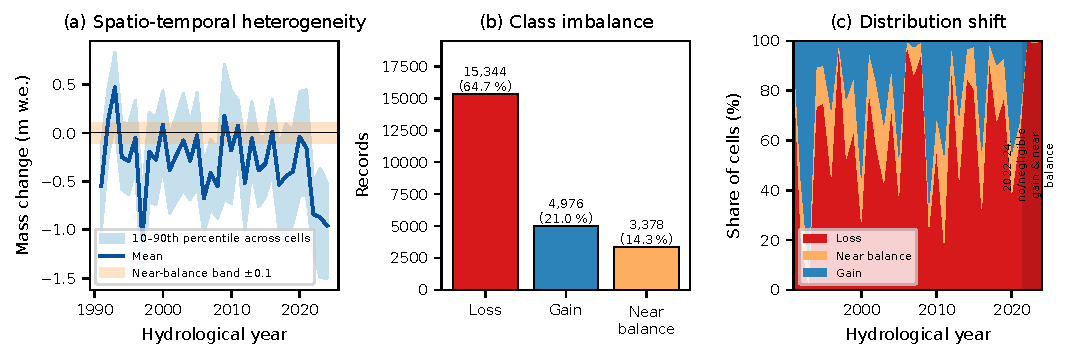
\includegraphics[width=\textwidth]{fig_problem_statement.pdf}
\caption{Problem statement. (a) Annual mass change is heterogeneous across cells: the band spans the 10th to 90th percentile and the shaded strip marks the near-balance interval. (b) The three classes are unequally represented. (c) The class mix shifts over time, with gain and near-balance cells almost absent in 2022--2024, so a model trained on all years faces a changing distribution.}
\label{fig:problem}
\end{figure*}

Annual proportions shift sharply: 2022 has no gain or near-balance cells; 2023 has five near-balance cells and no gain; 2024 has one near-balance cell and no gain. These years occur in both sides of spatial folds, so the shift is a non-stationarity issue rather than a temporal holdout.

\begin{figure}[t]
\centering
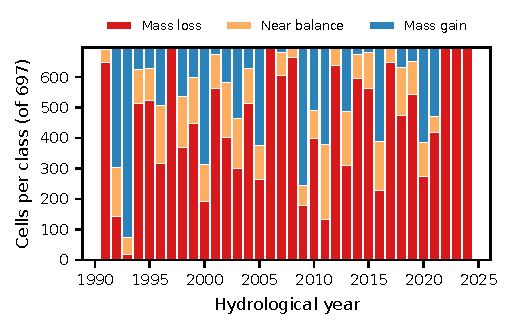
\includegraphics[width=\columnwidth]{fig_class_per_year.pdf}
\caption{Cells per class and hydrological year (697 cells per year). The scarcity of gain and near-balance cells after 2021 illustrates temporal distribution shift.}
\label{fig:perYear}
\end{figure}

\subsection{Label uncertainty}
Fig.~\ref{fig:uncert} compares the labels with the reported uncertainty. The median uncertainty (0.186~\mwe) exceeds the class half-width (0.1~\mwe), and 66.5\% of all records have an uncertainty above 0.1~\mwe. In 32.2\% of records the absolute value of the estimate is no larger than its own uncertainty, which includes 85.8\% of near-balance records. In 41.7\% of records the distance from the estimate to the nearest class boundary is within one reported uncertainty, so those records could plausibly belong to a neighbouring class. These shares were computed directly from the prepared table. They assume the uncertainty column is a one-sigma interval, which I could not confirm from the supplied documentation. Whatever its exact definition, the diagnostic implies that a large fraction of labels, and nearly all near-balance labels, are not statistically separable from their neighbours, and the near-balance class should be expected to be the hardest.

\begin{figure*}[t]
\centering
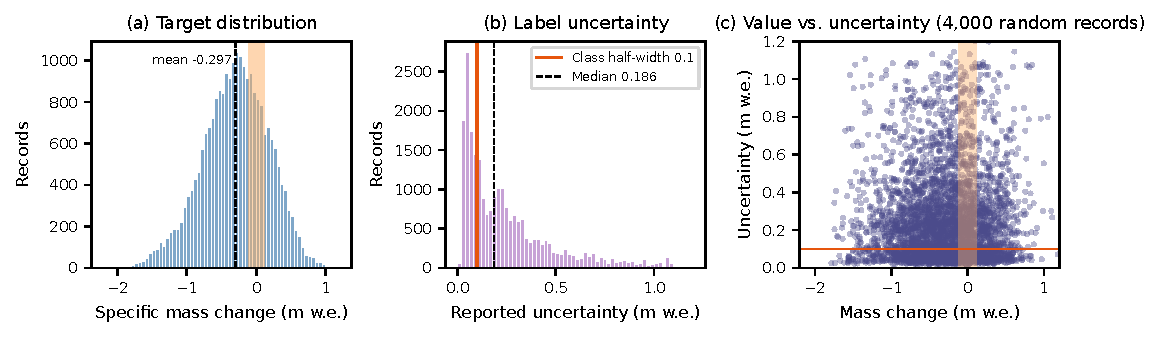
\includegraphics[width=\textwidth]{fig_target_uncertainty.pdf}
\caption{Target and label uncertainty. (a) Distribution of specific mass change with the near-balance band shaded. (b) Distribution of reported uncertainty with the class half-width marked. (c) Mass change against reported uncertainty for 4,000 random records; many records fall inside the shaded band with uncertainty above the 0.1 line.}
\label{fig:uncert}
\end{figure*}

\subsection{Hyperparameter search and selection}
Table~\ref{tab:params} lists the compact grids. The search comprises $3+8+2+8=21$ configurations and 105 fits, using the same five folds for every candidate. The best configuration per family is the one with the highest mean validation macro-F1, with balanced accuracy and accuracy as tie-breakers. The random seed is 42 in every component (clustering, fold assignment, estimators). The analysis used Python with scikit-learn, pandas and NumPy; version numbers are recorded in the experiment metadata and the notebook environment and should be listed in a release.

\begin{table}[t]
\caption{Search grids and selected configurations (21 candidates, 105 fits).}
\label{tab:params}
\centering
\footnotesize
\setlength{\tabcolsep}{3pt}
\begin{tabular}{p{0.20\columnwidth}p{0.36\columnwidth}p{0.30\columnwidth}}
\toprule
Classifier & Search values (configs) & Selected\\
\midrule
LR & $C\in\{0.1,1,10\}$ (3) & $C=10$\\
SVM (RBF) & $C\in\{1,5\}$; $\gamma=$ scale (2) & $C=5$; $\gamma=$ scale\\
RF & trees 150/300; depth 12/none; leaf 1/3 (8) & 300 trees; depth 12; leaf 3\\
GB & trees 100/200; rate 0.05/0.1; depth 2/3 (8) & 200 trees; rate 0.1; depth 3\\
\bottomrule
\end{tabular}
\end{table}

The grids are small. The same caution applies to search procedures: no optimiser outperforms all others over all possible objectives \cite{wolpert1997}, so the compact grid is a pragmatic choice and not a claim of optimality. The selected Gradient Boosting setting lies at the upper edge of all three searched ranges (200 trees, rate 0.1, depth 3), and the selected SVM cost is the larger of two values, so the optimum may lie outside the grid. LR has a single hyperparameter and the three values give almost identical scores (0.4035 to 0.4042 mean fold macro-F1), so LR's low score reflects model capacity and not under-tuning.

\subsection{Reporting protocol}
Model selection uses mean validation macro-F1 over the five folds. Pooled OOF predictions are then produced by refitting the selected configuration in each fold. Because the same folds serve selection and reporting, the pooled values are selection-fold diagnostics and not an independent test. A final Gradient Boosting model was also fitted on all 23,698 records and saved, but its fit is not an evaluation. No test partition, nested loop or chronological holdout exists in this experiment.

\section{Results}\label{sec:results}
\subsection{Model comparison}
Gradient Boosting ranked first on every summary (Table~\ref{tab:oof}, Fig.~\ref{fig:mc}). Pooled OOF accuracy was 0.6839 for Gradient Boosting, 0.6476 for Random Forest, 0.5192 for SVM and 0.5119 for Logistic Regression. Balanced accuracy and macro-F1 give the same order (0.6297 and 0.6037 for Gradient Boosting, 0.5382 and 0.5294 for Random Forest, 0.4747 and 0.4471 for SVM, 0.4368 and 0.4180 for Logistic Regression), and so does macro one-vs-rest ROC-AUC (0.8373, 0.7654, 0.6796, 0.6526).

\begin{table}[t]
\caption{Pooled spatial OOF metrics for each selected classifier. Selection-fold diagnostics, not independent test scores.}
\label{tab:oof}
\centering
\scriptsize
\setlength{\tabcolsep}{2pt}
\begin{tabular}{lrrrrr}
\toprule
Classifier & Acc. & Bal. acc. & Macro-F1 & Macro AUC & Macro prec.\\
\midrule
Gradient Boosting & 0.6839 & 0.6297 & 0.6037 & 0.8373 & 0.6058\\
Random Forest & 0.6476 & 0.5382 & 0.5294 & 0.7654 & 0.5244\\
SVM (RBF) & 0.5192 & 0.4747 & 0.4471 & 0.6796 & 0.4621\\
Logistic Regression & 0.5119 & 0.4368 & 0.4180 & 0.6526 & 0.4251\\
\bottomrule
\end{tabular}
\end{table}

\begin{figure}[t]
\centering
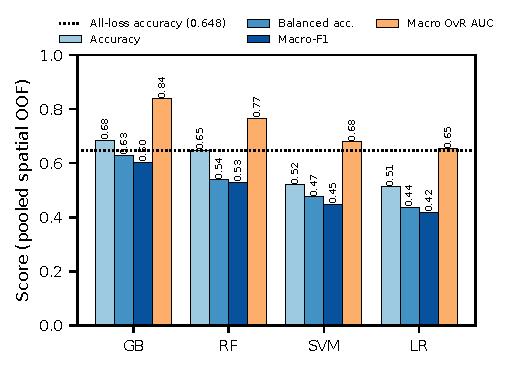
\includegraphics[width=\columnwidth]{fig_model_comparison.pdf}
\caption{Pooled spatial OOF accuracy, balanced accuracy, macro-F1 and macro ROC-AUC for the four classifiers. The dotted line marks the all-loss accuracy.}
\label{fig:mc}
\end{figure}

The all-loss rule already achieves 0.6475 accuracy. RF (0.6476) is essentially tied with it, while GB reaches 0.6839. Accuracy alone therefore obscures minority-class performance; balanced accuracy and macro-F1 provide the more informative ranking.

Mean fold macro-F1 was 0.5959 (SD 0.0506) for GB, 0.5228 (0.0359) for RF, 0.4315 (0.0289) for SVM and 0.4042 (0.0263) for LR. GB ranked first in all five folds, although its fold range (0.523--0.658) shows meaningful geographic variation.

\begin{table}[t]
\caption{Best configuration per family under five-fold spatial-group validation (mean over folds; SD of macro-F1 over the five folds).}
\label{tab:fold}
\centering
\scriptsize
\setlength{\tabcolsep}{2pt}
\begin{tabular}{lrrrr}
\toprule
Classifier & Macro-F1 (SD) & Bal. acc. & Acc. & Train F1\\
\midrule
Gradient Boosting & 0.5959 (0.0506) & 0.6292 & 0.6881 & 0.7146\\
Random Forest & 0.5228 (0.0359) & 0.5326 & 0.6557 & 0.7957\\
SVM (RBF) & 0.4315 (0.0289) & 0.4637 & 0.5259 & 0.5276\\
Logistic Regression & 0.4042 (0.0263) & 0.4304 & 0.5199 & 0.4336\\
\bottomrule
\end{tabular}
\end{table}

\begin{figure}[t]
\centering
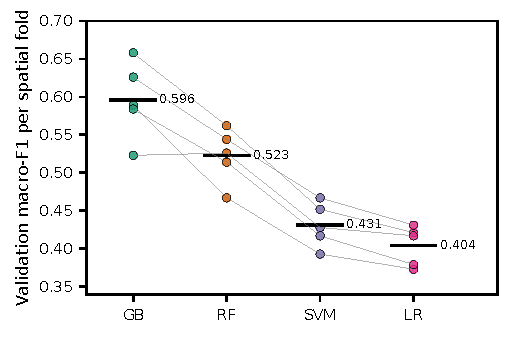
\includegraphics[width=\columnwidth]{fig_fold_scores.pdf}
\caption{Validation macro-F1 in each of the five spatial folds for the selected configurations (dots), with fold means (bars) and lines connecting the same fold across models. Fold ordering of the models is stable even though the absolute level changes.}
\label{fig:folds}
\end{figure}

\subsection{Class-wise performance}
The headline scores hide the main weakness (Table~\ref{tab:class}, Figs.~\ref{fig:cm} and \ref{fig:pc}). For Gradient Boosting, mass loss has F1 0.81 (precision 0.91, recall 0.73), mass gain 0.65 (precision 0.64, recall 0.66) and near balance 0.35 (precision 0.27, recall 0.50). Near balance recall of 0.50 means half of these records were recovered, but precision of 0.27 means that about three in four records predicted as near balance belong elsewhere. The confusion matrix (Fig.~\ref{fig:cm}) shows where the errors come from: of 15,344 true loss records, Gradient Boosting predicted 3,120 (20\%) as near balance and 969 (6\%) as gain. Because loss is large, those 3,120 records account for most of the false near-balance predictions, which outnumber the 1,687 true near-balance records that were correctly found. Of the 4,976 gain records, 1,352 (27\%) were predicted as near balance. The class is thus the sink for ambiguity from both sides, which agrees with the label-uncertainty diagnostic.

\begin{table}[t]
\caption{Pooled spatial OOF class-wise precision, recall and F1 of all four classifiers.}
\label{tab:class}
\centering
\scriptsize
\setlength{\tabcolsep}{2.5pt}
\begin{tabular}{lrrrrrrrrr}
\toprule
& \multicolumn{3}{c}{Mass gain} & \multicolumn{3}{c}{Mass loss} & \multicolumn{3}{c}{Near balance}\\
\cmidrule(lr){2-4}\cmidrule(lr){5-7}\cmidrule(lr){8-10}
Classifier & P & R & F1 & P & R & F1 & P & R & F1\\
\midrule
GB & 0.64 & 0.66 & 0.65 & 0.91 & 0.73 & 0.81 & 0.27 & 0.50 & 0.35\\
RF & 0.51 & 0.57 & 0.54 & 0.82 & 0.75 & 0.78 & 0.24 & 0.29 & 0.26\\
SVM & 0.37 & 0.47 & 0.42 & 0.82 & 0.56 & 0.67 & 0.19 & 0.39 & 0.26\\
LR & 0.32 & 0.49 & 0.39 & 0.78 & 0.58 & 0.67 & 0.17 & 0.24 & 0.20\\
Support & \multicolumn{3}{c}{4,976} & \multicolumn{3}{c}{15,344} & \multicolumn{3}{c}{3,378}\\
\bottomrule
\end{tabular}
\end{table}

\begin{figure*}[t]
\centering
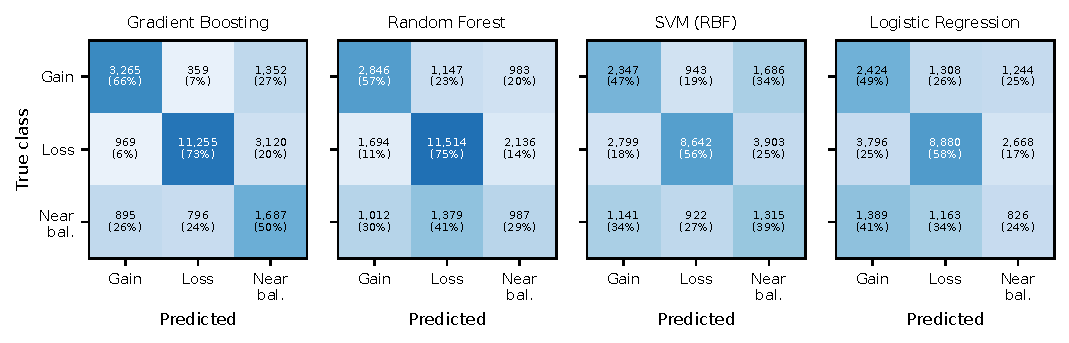
\includegraphics[width=\textwidth]{fig_confusion.pdf}
\caption{Pooled spatial OOF confusion matrices. Cells show counts and the row-normalised share of each true class. Counts were read from the validation notebook output and each matrix sums to the class supports in Table~\ref{tab:class}.}
\label{fig:cm}
\end{figure*}

\begin{figure*}[t]
\centering
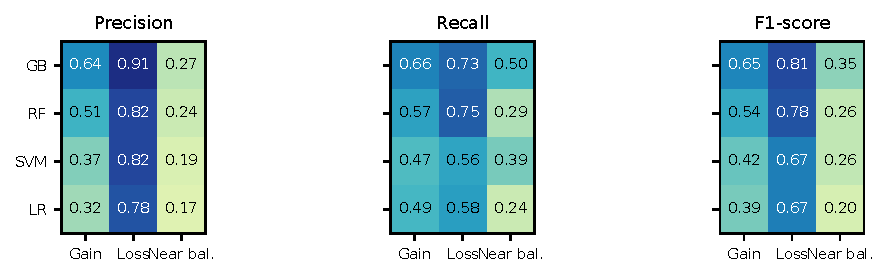
\includegraphics[width=\textwidth]{fig_perclass.pdf}
\caption{Class-wise precision, recall and F1 for the four classifiers. Near balance is the weakest class for every model, and precision is the weakest component for that class.}
\label{fig:pc}
\end{figure*}

No other model exceeds near-balance F1 of 0.26; recall ranges from 0.24 for LR to 0.50 for GB. Gain precision is also weaker for the linear and kernel models.

\subsection{ROC analysis}
One-vs-rest ROC-AUC for Gradient Boosting is 0.900 for gain, 0.886 for loss and 0.726 for near balance (Fig.~\ref{fig:roc} and Fig.~\ref{fig:auc}). The ranking of the three classes by AUC mirrors their ranking by F1, so the weakness on near balance is a ranking weakness as well as a threshold effect. A positive point for the model is that the gain and loss scores separate the classes well over thresholds. Because AUC measures ranking over all thresholds, whereas precision and recall depend on the classifier's decision rule, the two summaries need not agree; here they do.

\begin{figure}[t]
\centering
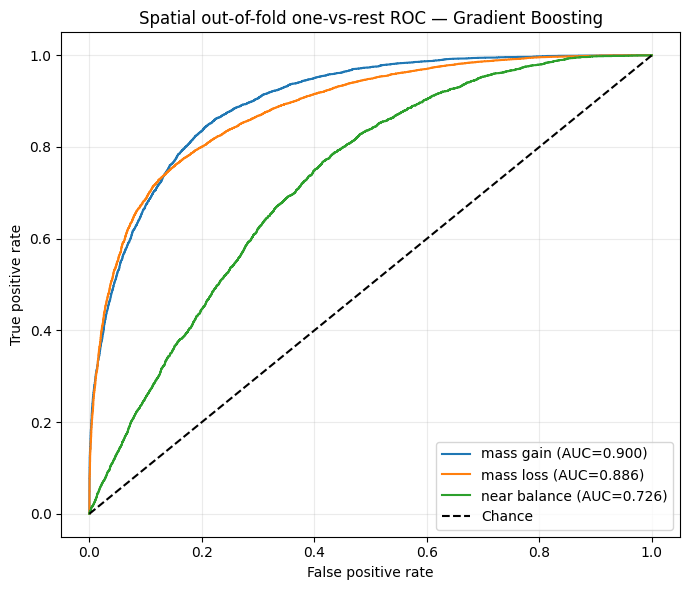
\includegraphics[width=0.92\columnwidth]{roc_gradient_boosting.png}
\caption{One-vs-rest ROC curves from pooled spatial OOF scores for Gradient Boosting (notebook output).}
\label{fig:roc}
\end{figure}

\begin{figure}[t]
\centering
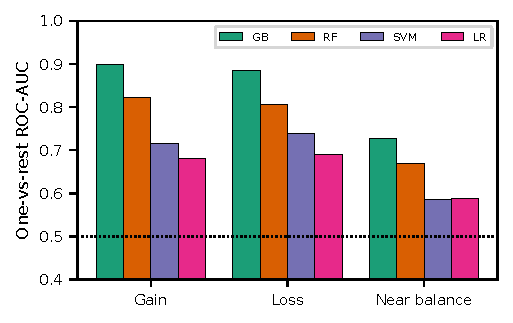
\includegraphics[width=\columnwidth]{fig_auc_class.pdf}
\caption{Class-wise one-vs-rest ROC-AUC for all classifiers. The dotted line marks chance (0.5); near-balance AUC for SVM and Logistic Regression is only 0.58--0.59.}
\label{fig:auc}
\end{figure}

\subsection{Training versus validation and hyperparameter sensitivity}
Training--validation macro-F1 gaps were 0.27 for RF (0.7957 versus 0.5228), 0.12 for GB, 0.10 for SVM and 0.03 for LR. Unrestricted RF trees reached perfect training fit but substantially lower validation scores. GB's searched scores increased with estimator count, learning rate and depth; its optimum lies at the upper edge of the grid, so a broader search is warranted rather than assuming the reported setting is globally optimal.

\begin{figure}[t]
\centering
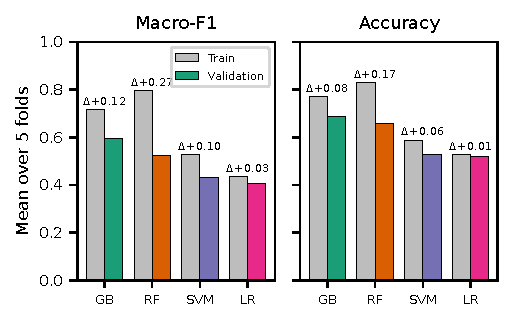
\includegraphics[width=\columnwidth]{fig_train_val.pdf}
\caption{Mean training and validation macro-F1 and accuracy over five spatial folds for the selected configurations. Labels show the training minus validation difference.}
\label{fig:tv}
\end{figure}

\begin{figure*}[t]
\centering
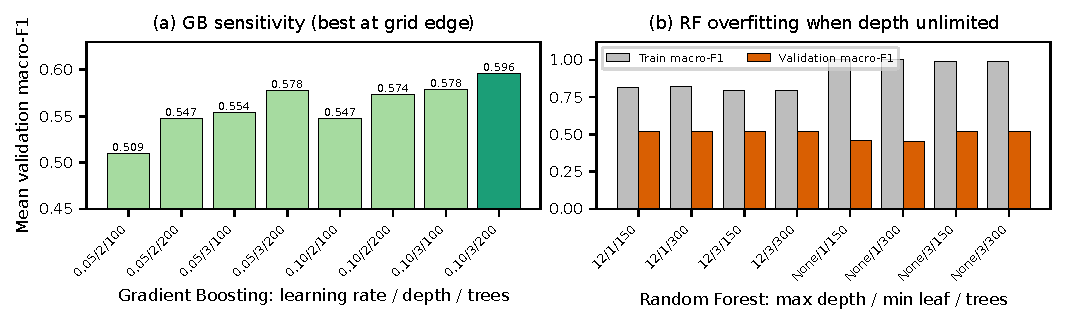
\includegraphics[width=\textwidth]{fig_hyperparam.pdf}
\caption{Hyperparameter sensitivity of mean validation macro-F1. (a) The eight Gradient Boosting configurations; the best lies at the upper edge of the grid. (b) The eight Random Forest configurations, with training and validation scores; unlimited depth reproduces the training data but not the validation clusters.}
\label{fig:hp}
\end{figure*}

\subsection{Computational cost}\label{sec:cost}
The single-run notebook log gives per-fit times of about 0.05 min for LR, 0.49 min for RF, 1.05 min for SVM and 1.58 min for GB. Thus GB took about 34 times as long as LR while increasing pooled macro-F1 by 0.19. The final all-record GB fit took 196.67 s and produced a 0.75 MB artifact. Hardware was not recorded; memory was not profiled and timings were not repeated, so these values are indicative only.

\begin{table}[t]
\caption{Measured wall-clock cost from the logged search (indicative; unspecified hosted hardware).}
\label{tab:cost}
\centering
\scriptsize
\setlength{\tabcolsep}{2.5pt}
\begin{tabular}{lrrrr}
\toprule
Classifier & Fits & Search time (min) & Per fit (min) & Macro-F1 (OOF)\\
\midrule
Logistic Regression & 15 & 0.7 & 0.05 & 0.4180\\
Random Forest & 40 & 19.5 & 0.49 & 0.5294\\
SVM (RBF) & 10 & 10.5 & 1.05 & 0.4471\\
Gradient Boosting & 40 & 63.3 & 1.58 & 0.6037\\
Total search & 105 & 94.0 & 0.90 & --\\
\bottomrule
\end{tabular}
\end{table}

\begin{figure}[t]
\centering
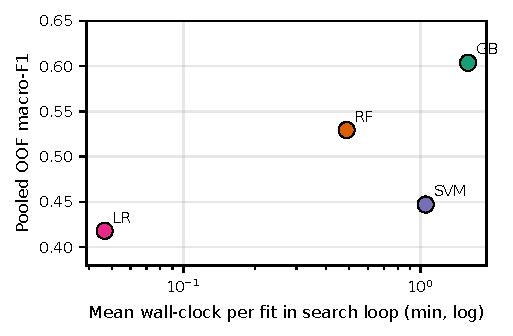
\includegraphics[width=\columnwidth]{fig_cost_perf.pdf}
\caption{Performance versus logged cost: pooled OOF macro-F1 against mean wall-clock time per fit (log scale). Times come from one run on unspecified hardware.}
\label{fig:cost}
\end{figure}

\subsection{Predictor behaviour by class}
Box plots of selected predictors by class (Fig.~\ref{fig:pred}) show overlap rather than clean separation. Median annual 2-m temperature is 266.6~K for gain, 267.2~K for near balance and 268.0~K for loss, so colder cells are more often gaining, but the interquartile ranges overlap strongly. Median snow cover is 37.8 for gain, 38.5 for near balance and 42.7 for loss, a counter-intuitive ordering (more snow cover in loss cells) that is plausible only because cells differ in location and elevation, and it illustrates why pooled correlation is not causal. The weak univariate separation is consistent with the modest scores of linear models and with the larger gain from nonlinear interactions.

\begin{figure*}[t]
\centering
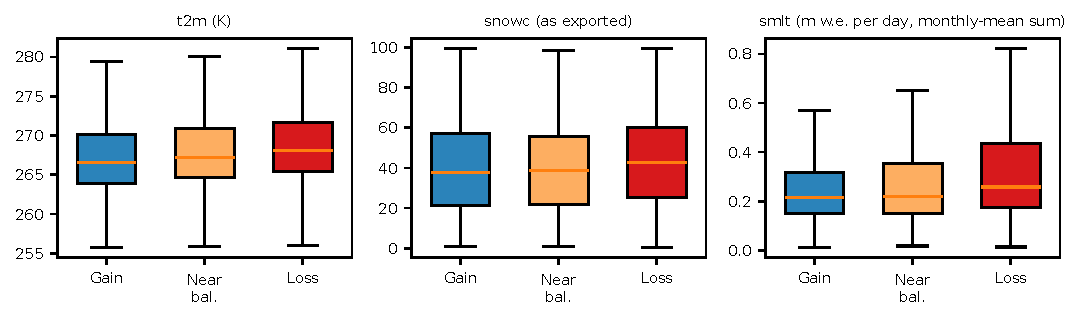
\includegraphics[width=\textwidth]{fig_predictors_by_class.pdf}
\caption{Distribution of annual 2-m temperature, snow cover and snowmelt by target class (outliers hidden). Distributions overlap strongly, so no single predictor separates the classes.}
\label{fig:pred}
\end{figure*}

\subsection{A diagnostic on replaced ERA5-Land months}\label{sec:diag}
Fig.~\ref{fig:disc} plots annual means of three climate variables across the whole grid. Before 2022, annual mean 2-m temperature is $268.54\pm0.49$~K (mean and standard deviation of 1991--2021). In hydrological year 2022, which contains no replaced months, it is 268.75~K ($+0.42$ SD). In 2023, with seven replaced months, it is 267.14~K ($-2.85$ SD), and in 2024, with eleven replaced months, it is 264.70~K ($-7.79$ SD). Annual mean zonal wind \texttt{u10} falls from $0.54\pm0.05$ to 0.278 and 0.199~m\,s$^{-1}$, that is $-5.5$ and $-7.1$ SD. Annual precipitation, in contrast, stays within one standard deviation of the earlier mean ($+0.60$ and $-0.67$ SD), and net solar radiation is $+2.15$ SD in 2023 and $+0.72$ SD in 2024.

\begin{figure*}[t]
\centering
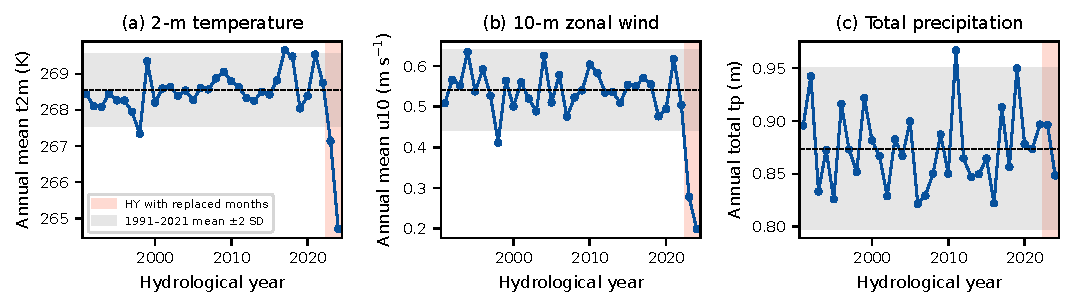
\includegraphics[width=\textwidth]{fig_era5_discontinuity.pdf}
\caption{Grid-mean annual (a) 2-m temperature, (b) 10-m zonal wind and (c) total precipitation by hydrological year. The shaded red band marks the two years that contain replaced months; the grey band is the 1991--2021 mean $\pm2$ standard deviations.}
\label{fig:disc}
\end{figure*}

A 3.8~K annual temperature drop across 697 cells coincides with the replaced months and is not a plausible regional climate signal. One possible explanation is that 00:00 values replaced monthly means for \texttt{t2m} and wind, but this hypothesis was not tested against original monthly values. HY2023 and HY2024 contain 1,394 records (5.9\% of the table) and also have almost no gain or near-balance labels. The classifier could therefore learn an artefactual association between these years, anomalous climate inputs and the loss class. The resulting contamination risk is unquantified.

\subsection{Supplementary chronological imbalance experiment}
A second notebook, \path{glacier_mass_change_integrated_hkh_ml.ipynb}, tests class-imbalance strategies under a different design. It uses 19 predictors, including latitude and longitude, and separates 1991--2019 for development from an untouched 2020--2024 test period. Six expanding-window validation folds use progressively longer training periods. Four algorithms (LR, RBF-SVM, RF and XGBoost) are each tested with four settings: neither undersampling nor weighting, undersampling only, weighting only, and both. Four parameter samples per algorithm--strategy combination yield 64 candidates and 384 fold fits. Undersampling is applied only to training folds using \texttt{RandomUnderSampler}; validation and test records retain their natural class distribution. Balanced class weights are computed from the original training fold. For XGBoost, those weights are passed as sample weights.

The selected configuration is LR with class weighting and no undersampling, because it has the highest mean expanding-window validation macro-F1 (0.3443). Its test macro-F1 is 0.2535, balanced accuracy 0.3066 and accuracy 0.4772. The best validation-ranked RF configuration without either imbalance treatment has test macro-F1 0.3587, balanced accuracy 0.3546 and accuracy 0.7145. This reversal is reported rather than used to change the selected model: the notebook chooses by validation macro-F1 and then evaluates the test set. The results also show why the test set must not be used to retrospectively choose a different strategy.

Table~\ref{tab:imbalance} summarises the highest validation-ranked configuration within each imbalance strategy. Because the algorithm can differ between rows, this is a comparison of the best observed strategy--model combinations, not a controlled causal estimate of the effect of resampling or weighting alone. The notebook uses one fixed seed and only four sampled parameter settings per combination; strategy differences should therefore be treated as exploratory. This experiment is kept separate from the primary spatial experiment: its 19-feature set, temporal split and four-algorithm search are not interchangeable with the spatial notebook's 17-feature, 25-cluster evaluation.

\begin{table*}[t]
\caption{Chronological experiment: best validation-ranked model configuration within each imbalance strategy.}
\label{tab:imbalance}
\centering\scriptsize
\setlength{\tabcolsep}{2pt}
\begin{tabular}{p{0.11\textwidth}p{0.12\textwidth}p{0.09\textwidth}p{0.09\textwidth}p{0.11\textwidth}p{0.09\textwidth}p{0.30\textwidth}}
\toprule
Strategy & Selected algorithm & Val. macro-F1 & Test macro-F1 & Test balanced acc. & Test accuracy & Practical interpretation\\
\midrule
Neither & RF & 0.3387 & 0.3587 & 0.3546 & 0.7145 & Retains natural training distribution; best test score among the 16 selected configurations, but not the top validation result.\\
Undersampling only & LR & 0.3406 & 0.2489 & 0.2976 & 0.4631 & Reduces majority examples in training; may discard useful majority-class variation.\\
Class weighting only & LR & 0.3443 & 0.2535 & 0.3066 & 0.4772 & Retains all training observations and penalises minority errors more; highest validation macro-F1 and selected by the notebook.\\
Both & RF & 0.3268 & 0.3055 & 0.3344 & 0.5214 & Combines reduced sample size with original-fold weights; can amplify minority influence and performed below the best single treatment here.\\
\bottomrule
\end{tabular}
\end{table*}

\begin{figure}[t]
\centering
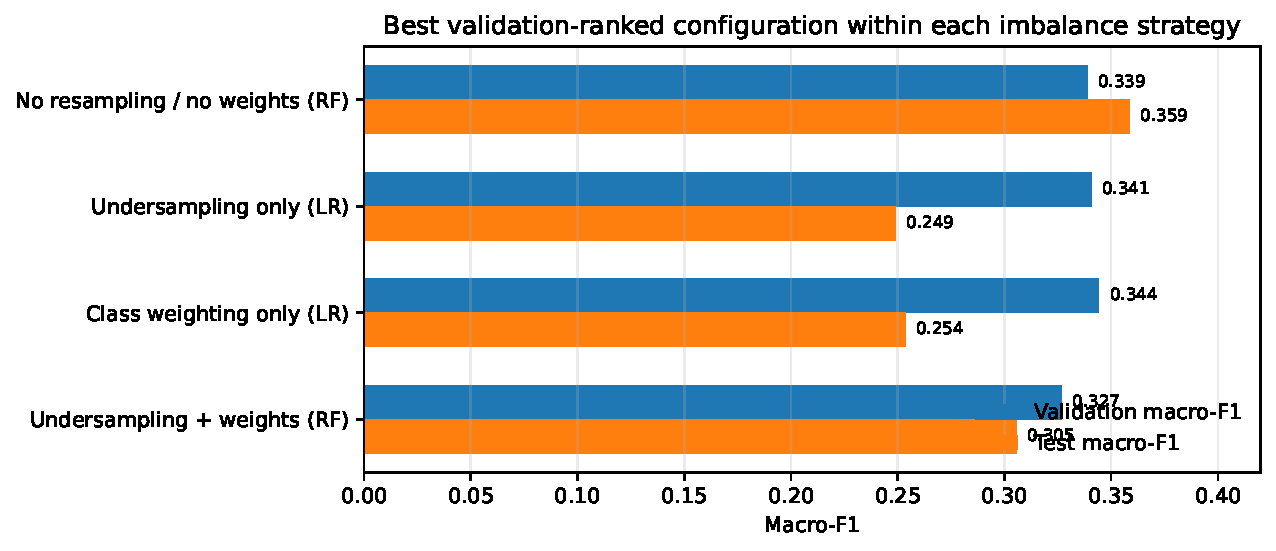
\includegraphics[width=\columnwidth]{fig_imbalance_comparison.pdf}
\caption{Validation and 2020--2024 test macro-F1 for the best validation-ranked model within each chronological imbalance strategy. The algorithm differs between strategies; this is not a controlled estimate of the isolated treatment effect.}
\label{fig:imbalance}
\end{figure}

The spatial experiment's final model uses class weighting without undersampling; the chronological experiment's selected LR configuration is a separate result and is not deployed in the supplied Streamlit application. The application README and model artifact identify the spatial Gradient Boosting estimator as the deployed model.

\section{Discussion}\label{sec:discussion}
\subsection{What the evidence supports}
Under shared spatially grouped folds, boosted trees give the best separation of the three classes, bagged trees are second, and kernel and linear models are clearly weaker. This ordering agrees in direction with the finding in the Alpine base study that nonlinear and tree-based learners beat a linear baseline and that ensemble trees are strong on medium-sized correlated tabular data \cite{anilkumar2023}, and with the use of boosting as the preferred learner in several High Mountain Asia studies \cite{gurung2025,peng2025,sjursen2025}. It does not agree on the second place: in the Alpine study the SVM was competitive with the forest, whereas here it was clearly below it. Differences in task (classification versus point regression), sample size, feature set and validation make this a comparison of tendencies, not of numbers. Regression scores such as R$^2$ and classification scores such as macro-F1 are not interchangeable, so I do not rank this paper against those papers.

\subsection{Why the weakest model is weak, and why boosting is strongest}
LR and SVM have small training--validation gaps but lower scores, consistent with limited capacity for nonlinear interactions among correlated climate predictors. RF can overfit when depth is unrestricted; depth and leaf-size limits reduce but do not remove that gap. GB performs best under the searched shallow-tree settings. No feature-importance analysis was run for the primary spatial experiment, so predictor-level attribution is not claimed. Strong correlations among snow, runoff and radiation variables would also make individual importance shares difficult to interpret \cite{anilkumar2023}.

\subsection{Near balance is a label problem as much as a model problem}
Near-balance weakness may reflect label ambiguity, class size, temporal scarcity and its transitional position between gain and loss. The strongest direct evidence is uncertainty: 85.8\% of near-balance records have estimates no larger than their reported uncertainty, whose median is nearly twice the class half-width. Gain is also a minority class but has higher F1 (0.65), so imbalance alone is insufficient. Only six near-balance records occur in the last three years. These diagnostics suggest an uncertainty-aware label sensitivity analysis, but do not isolate each cause.

\subsection{Spatial validation: what it does and does not show}
The grouped design removes repeated-location leakage, which is the largest obvious leakage in a panel of 697 locations by 34 years, and group separation is verified. It does not show geographic independence. The clusters are formed in standardised coordinate space, neighbouring clusters touch, and cells near a boundary share climate. Spatial dependence may therefore lower the apparent difficulty of transfer. Wadoux et al. caution that spatial cross-validation cannot replace probability-sample validation for map accuracy \cite{wadoux2021}, and Meyer and Pebesma stress that cross-validation error applies only inside the model's area of applicability \cite{meyer2021}; both points apply here. The folds also include all years, so the test is of spatial transfer within the observed period, and a model that exploits hydrological year can benefit from temporal structure shared by training and validation. A spatio-temporal blocked design, with a buffer and a chronological holdout, would address both limits.

The reuse of folds for tuning and reporting adds an optimistic bias that grows with the number of configurations compared. The effect is probably modest for the small grids here, particularly for LR and SVM, but it is probably larger for Gradient Boosting, where eight configurations are compared and the best of them is reported. This does not alter the ranking logic but it does mean that the absolute scores of the winning configurations are upper estimates. The pooled scores are also computed from predictions of models that were selected on the same data.

\subsection{Implications for HKH monitoring}
The classifier recovers mass-loss and mass-gain cells in held-out clusters with F1 scores of 0.81 and 0.65, but remains unreliable for near balance. Because inputs summarise the full target year and labels represent grid cells, this is retrospective cell-level screening, not forecasting or glacier-level inference.

\subsection{Relation to the blueprint}
The blueprint exposed the main departures: the executed scope is HKH rather than Nepal-only, the primary target is not uncertainty-aware, and the primary experiment has no locked temporal test. Priority follow-up is to verify and rerun the climate table, test alternative labels, and implement nested spatial and chronological evaluation.

\section{Threats to Validity and Limitations}\label{sec:threats}
Table~\ref{tab:threats} collects the principal threats by type, with the evidence in this paper and the action that would resolve each.

\begin{table*}[t]
\caption{Threats to validity, evidence in this study and resolving action.}
\label{tab:threats}
\centering
\footnotesize
\setlength{\tabcolsep}{3pt}
\begin{tabular}{p{0.12\textwidth}p{0.28\textwidth}p{0.27\textwidth}p{0.25\textwidth}}
\toprule
Type & Threat & Evidence here & Resolving action\\
\midrule
Internal & Same folds for tuning and reporting & Selection and pooled OOF scores share folds & Nested spatial CV or untouched spatial region\\
Internal & Spatial leakage across adjacent clusters & Cluster identity checked, distance not & Buffered blocks; sensitivity to $k$ (e.g., 15, 25, 35)\\
Internal & Time proxy through hydrological year & Year is a predictor; folds contain all years & Ablate year; chronological holdout\\
Internal & Grid-edge optima & GB best at upper edge of all three ranges & Extend grid or randomised search\\
Data & Replaced ERA5-Land months with unverified semantics & $-2.85$ and $-7.79$ SD temperature anomalies in 2023, 2024 & Keep original \texttt{t2m}, \texttt{u10}, \texttt{v10}; verify units; rerun\\
Data & Label ambiguity vs. uncertainty & Median $u=0.186>0.1$; 85.8\% of near-balance records & Uncertainty-aware labels; boundary exclusion test\\
Data & Uncertainty definition unknown & 1$\sigma$ vs 1.96$\sigma$, annual vs cumulative unconfirmed & Confirm in product documentation\\
Data & 9 km reanalysis over steep terrain; no elevation, aspect or debris & Predictors limited to climate, year and area & Add topographic features; compare with stations\\
External & Applies to 697 cells and 1991--2024 only & Panel is complete but a single product & Independent product or region\\
External & Retrospective, not a forecast & Same-year predictors & Lagged or forecast predictors with chronological test\\
Construct & Class thresholds are a convention & Fixed $\pm0.1$ & Report results for several $\tau$\\
Computational & Hardware-dependent, single-run timings & Unspecified hosted hardware; no memory profile & Repeated runs on recorded hardware\\
\bottomrule
\end{tabular}
\end{table*}

Claims are restricted to the supplied cells and years, not individual glaciers or the entire HKH. The uncertainty and climate discontinuity diagnostics are exploratory, and ERA5-Land aggregation rules and the exported snow-cover scale remain unverified against original NetCDF attributes.

\section{Conclusion and Future Work}\label{sec:conclusion}
This study compared LR, RBF-SVM, RF and GB on 23,698 HKH cell-year records. In five-fold validation on 25 coordinate clusters, GB led (mean fold macro-F1 0.5959; pooled OOF macro-F1 0.6037; balanced accuracy 0.6297; macro-AUC 0.8373), but near-balance F1 was only 0.35 and its accuracy exceeded the all-loss rule by about 3.6 percentage points. The median reported uncertainty (0.186~\mwe) exceeds the class half-width, and 85.8\% of near-balance estimates are no larger than their uncertainty. GB was also about 34 times slower per fit than LR in the logged run.

These results are retrospective, and the same spatial folds support tuning and reporting. The two years containing replaced ERA5-Land months show implausible anomalies and may contaminate 5.9\% of records. Uncertainty-aware labels and nested spatial validation remain open for the primary experiment.

Future work should proceed in this order. (1) Restore the original monthly values for non-accumulated variables, verify the recovery product's semantics for accumulated ones and rerun the table and the models. (2) Compare fixed, uncertainty-aware and boundary-excluded labels. (3) Add nested spatial validation with a buffer, a cluster-count sensitivity analysis and a chronological holdout. (4) Ablate year and area and add topographic predictors. (5) Extend the Gradient Boosting grid, add a no-weighting control and evaluate histogram-based boosting. (6) Repeat the cost measurements on recorded hardware with memory profiling. Until then, the classifier is best read as a documented starting point for screening-level work on HKH glacier mass-change state, not as an operational tool.

\section*{Acknowledgment}
This study uses modified Copernicus Climate Change Service information from 2019 and 2023. Neither the European Commission nor ECMWF is responsible for any use that may be made of the Copernicus information or data it contains. No human or animal subjects were involved.

\bibliographystyle{IEEEtran}
\bibliography{references}


\clearpage
\appendices
\section{Supplementary Part I: Code and Reproducibility}
\label{app:code}

\subsection*{A. Links}
\begin{itemize}
\item \textbf{Github repository:} \url{https://github.com/Code-With-Samuel/glacier_research}
\item \textbf{Research explanation video (YouTube):} \url{https://youtu.be/brRSi5CpUVU?si=kKkQe97-WWHAX-hf}
\end{itemize}

\subsection*{B. Code snippets}
The snippets are taken from the repository notebooks
(\texttt{supervised\_learning\_for\_classification},
\texttt{glacier\_mass\_change\_integrated\_hkh\_ml}) and the dashboard,
shortened only by omitting print statements and figure-generation code.

\begin{figure}[H]
\centering
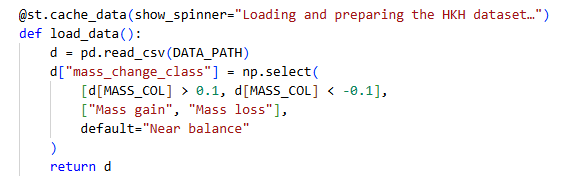
\includegraphics[width=\columnwidth]{code_screenshots/b1.png}
\caption{B.1 Target classes (dashboard loader, \texttt{app.py}).}
\label{fig:code-b1-target-classes}
\end{figure}

\begin{figure}[H]
\centering
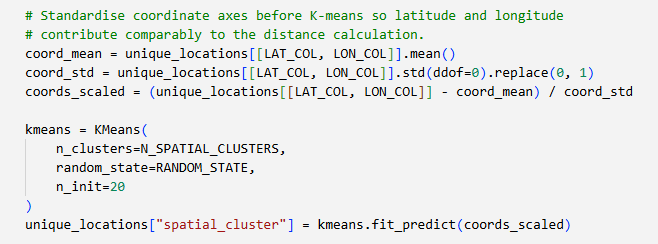
\includegraphics[width=\columnwidth]{code_screenshots/b2.png}
\caption{B.2 Spatial clusters (spatial-validation notebook).}
\label{fig:code-b2-spatial-clusters}
\end{figure}

\begin{figure}[H]
\centering
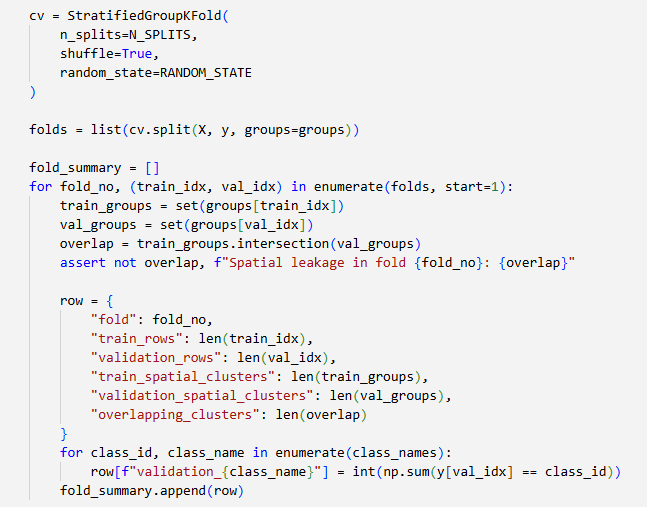
\includegraphics[width=\columnwidth]{code_screenshots/b3.png}
\caption{B.3 Grouped folds with leakage check (spatial-validation notebook).}
\label{fig:code-b3-grouped-folds}
\end{figure}

\begin{figure}[H]
\centering
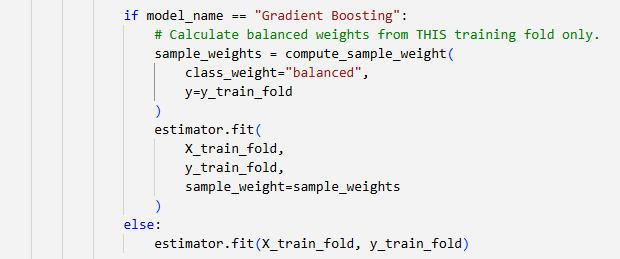
\includegraphics[width=\columnwidth]{code_screenshots/b4.png}
\caption{B.4 Fold-wise balanced weights for Gradient Boosting (spatial-validation notebook).}
\label{fig:code-b4-balanced-weights}
\end{figure}

\begin{figure}[H]
\centering
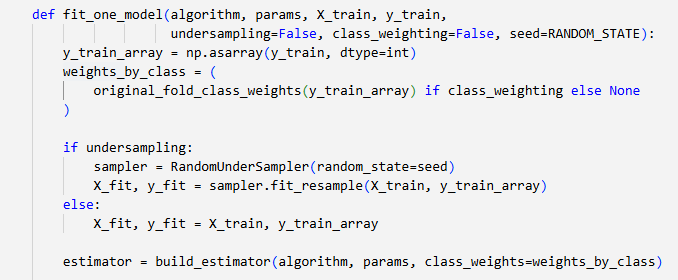
\includegraphics[width=\columnwidth]{code_screenshots/b5.png}
\caption{B.5 Imbalance settings (chronological notebook).}
\label{fig:code-b5-imbalance-settings}
\end{figure}

\begin{figure}[H]
\centering
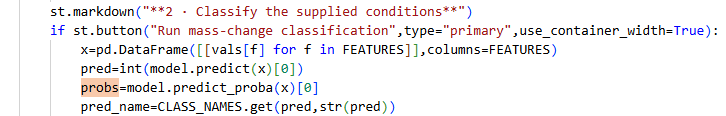
\includegraphics[width=\columnwidth]{code_screenshots/b6.png}
\caption{B.6 Prediction in the dashboard (\texttt{app.py}).}
\label{fig:code-b6-dashboard-prediction}
\end{figure}

\section{Supplementary Part II: Streamlit Application Demonstration}
\label{app:application}
The dashboard (\texttt{app.py}) was running locally for these captures on the supplied data and model. The interactive map pages use an online basemap through Folium; in the capture environment the map component did not render, so no map screenshot is shown.
\begin{figure}[H]
\centering
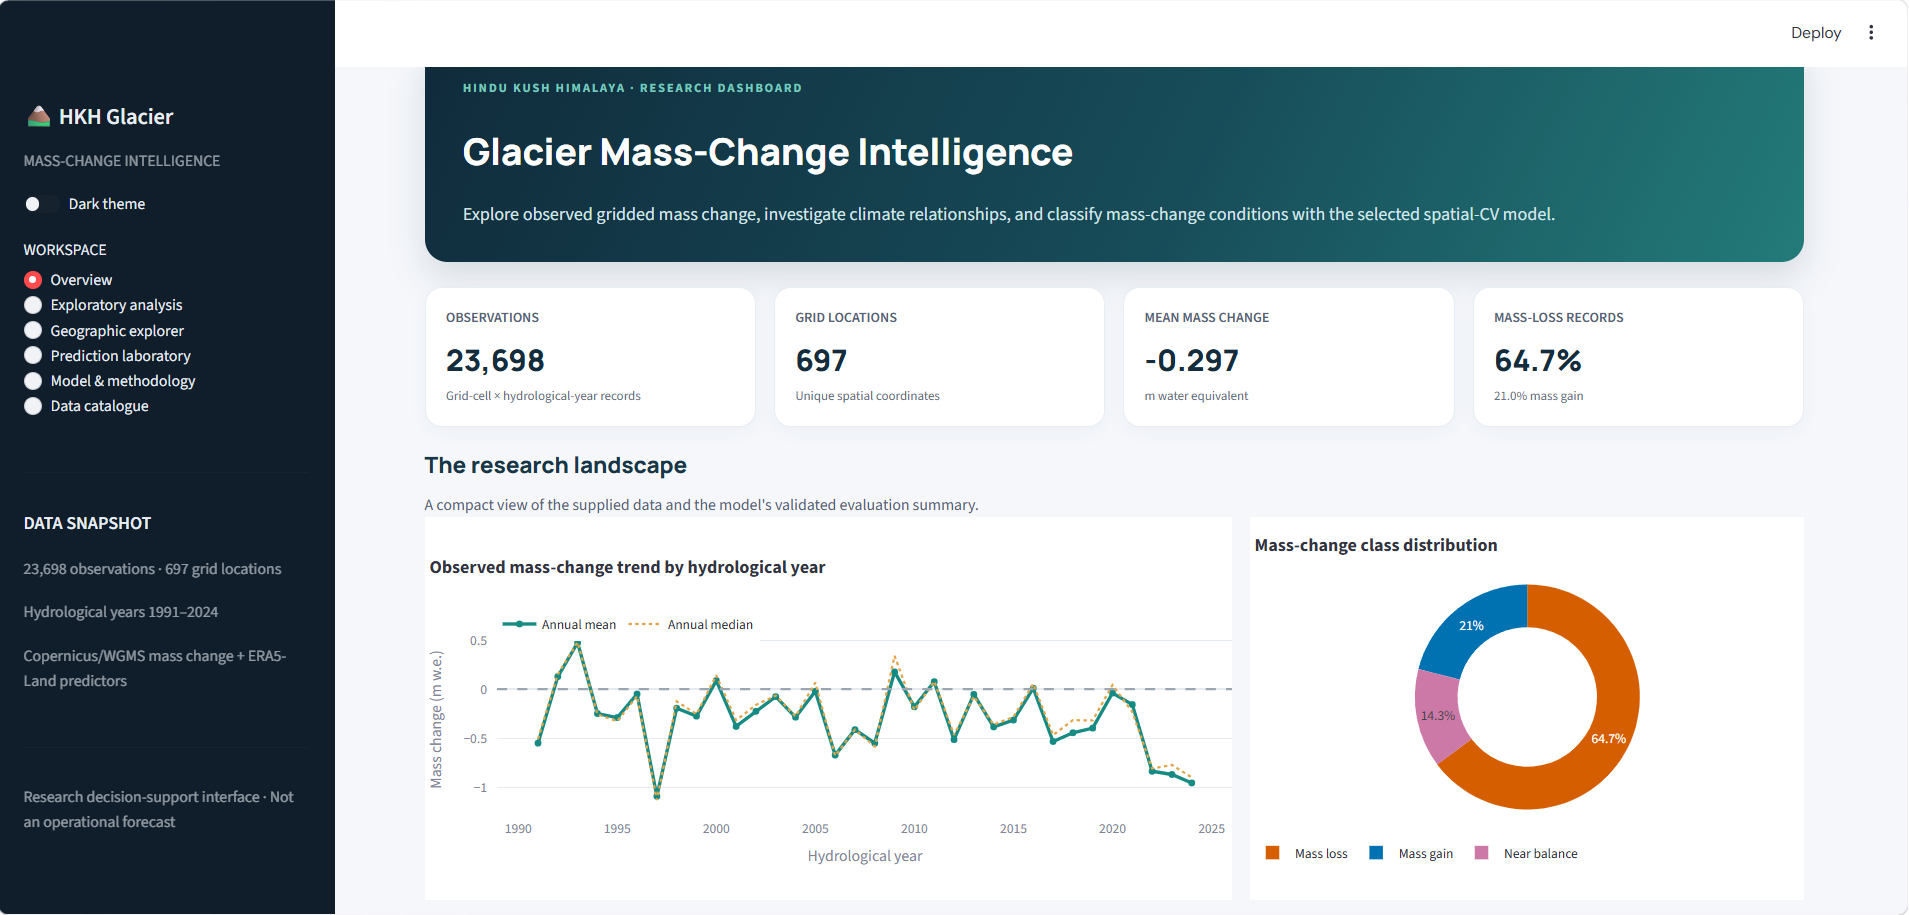
\includegraphics[width=\columnwidth]{dashboard_screenshots/overview.png}
\caption{Streamlit dashboard overview.}
\label{fig:dashboard-overview}
\end{figure}

\begin{figure}[H]
\centering
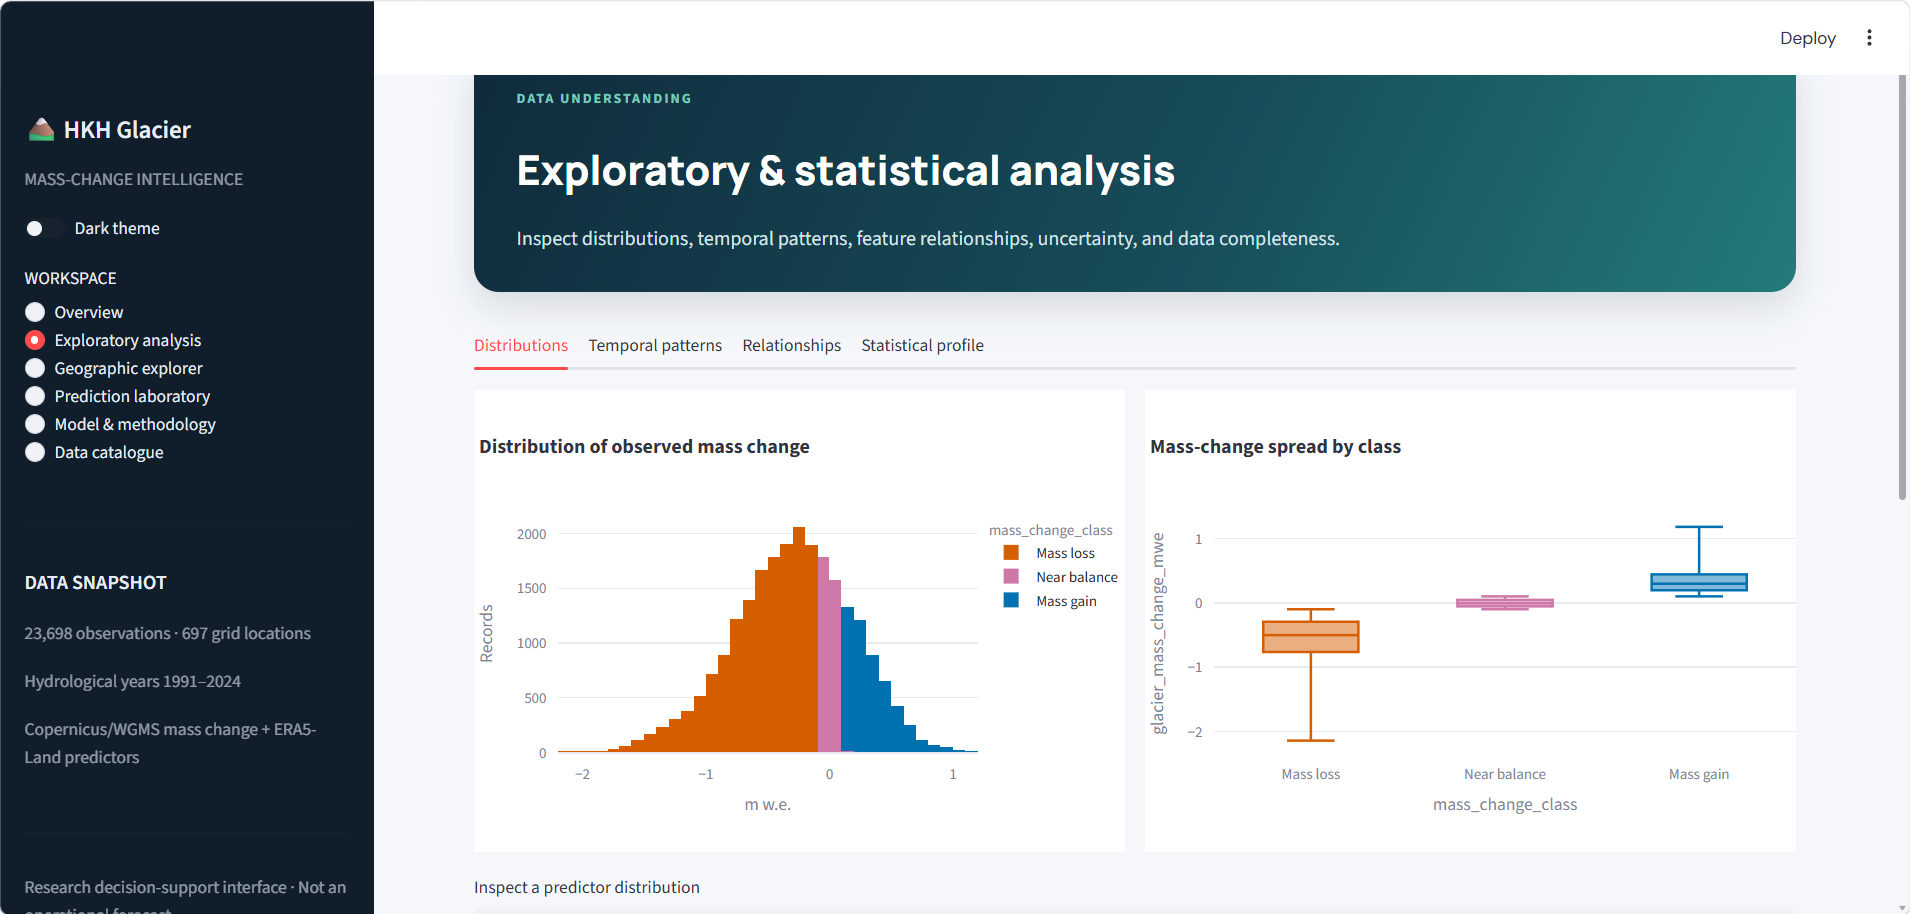
\includegraphics[width=\columnwidth]{dashboard_screenshots/exploratory_analysis_1.png}
\caption{Streamlit exploratory analysis: class distribution and summary view.}
\label{fig:dashboard-exploratory-1}
\end{figure}

\begin{figure}[H]
\centering
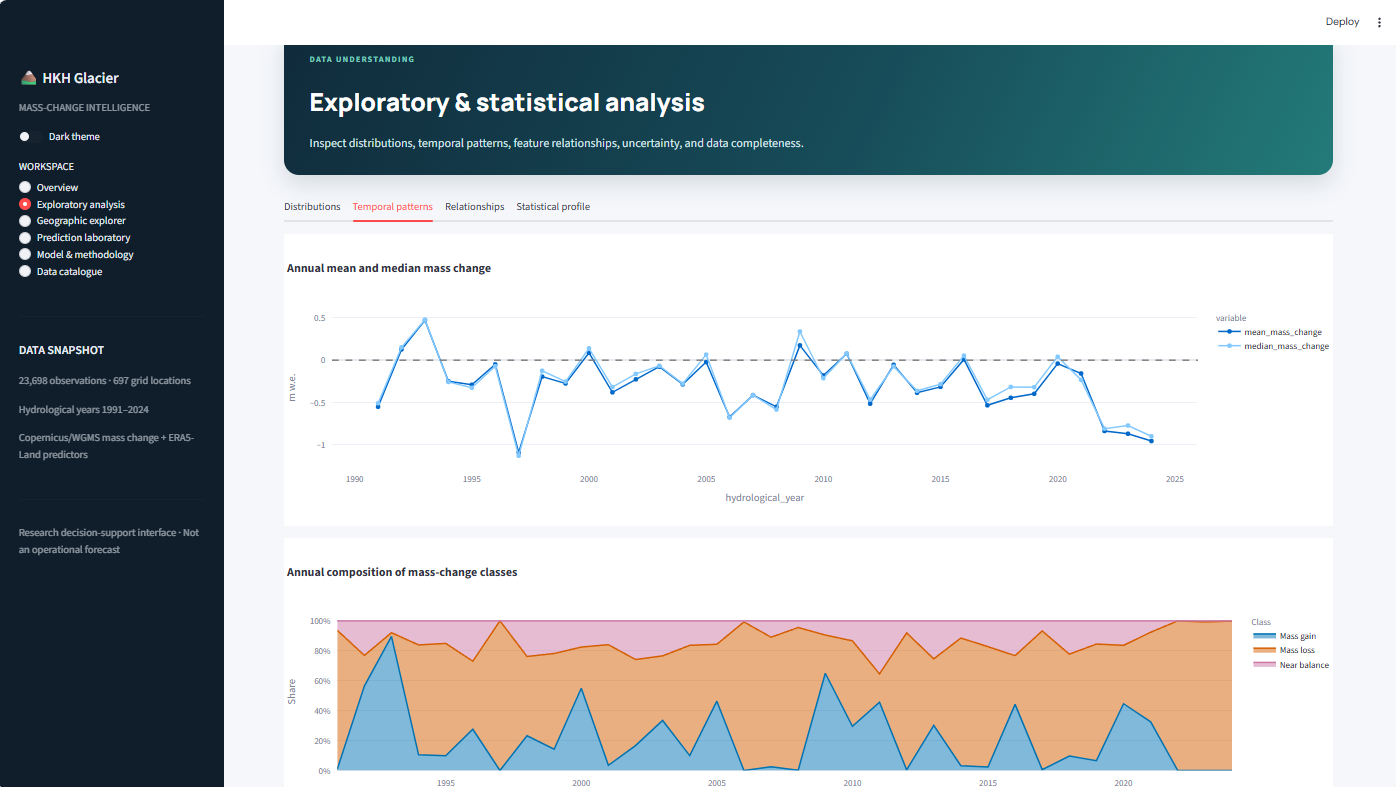
\includegraphics[width=\columnwidth]{dashboard_screenshots/exploratory_analysis_2.png}
\caption{Streamlit exploratory analysis: predictor comparison view.}
\label{fig:dashboard-exploratory-2}
\end{figure}

\begin{figure}[H]
\centering
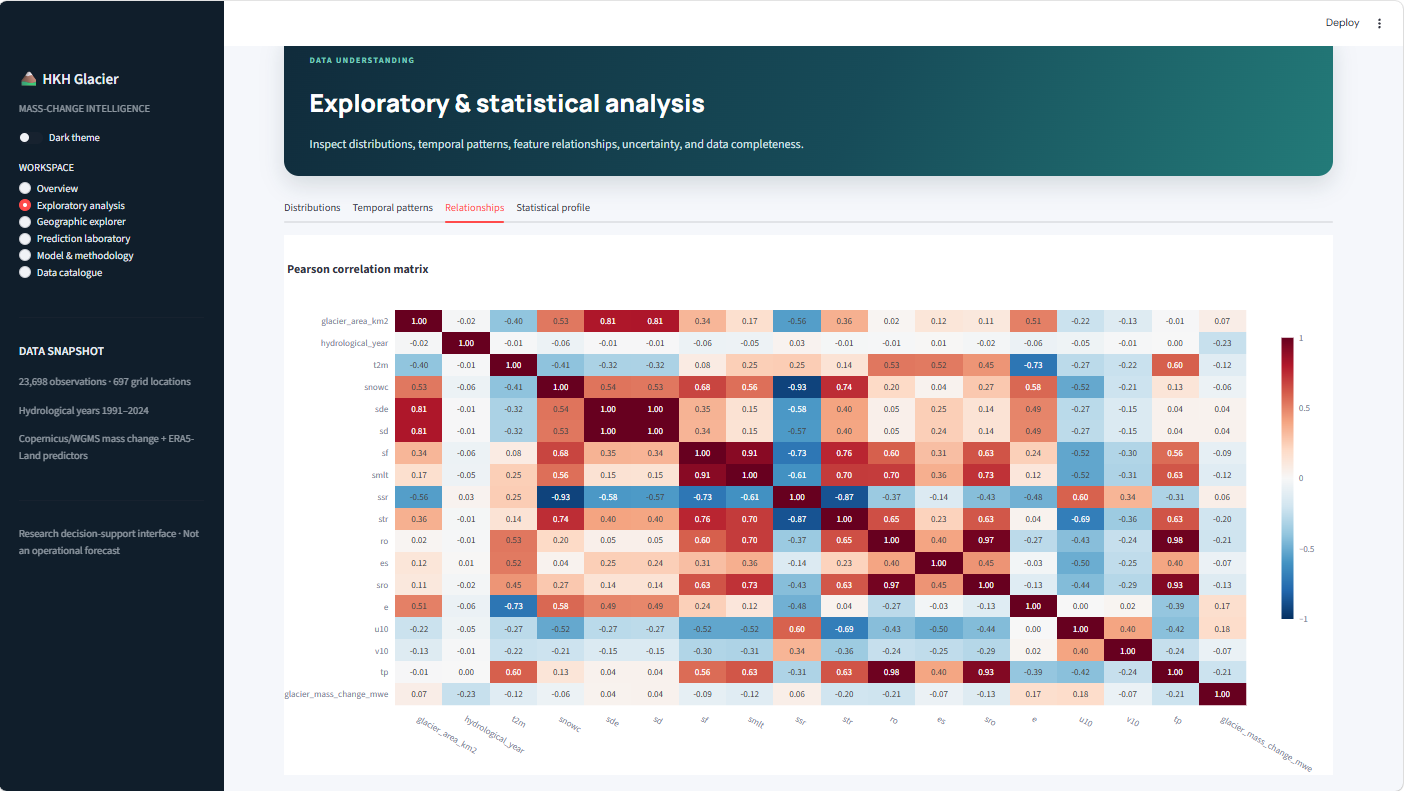
\includegraphics[width=\columnwidth]{dashboard_screenshots/exploratory_analysis_3.png}
\caption{Streamlit exploratory analysis: additional diagnostic view.}
\label{fig:dashboard-exploratory-3}
\end{figure}

\begin{figure}[H]
\centering
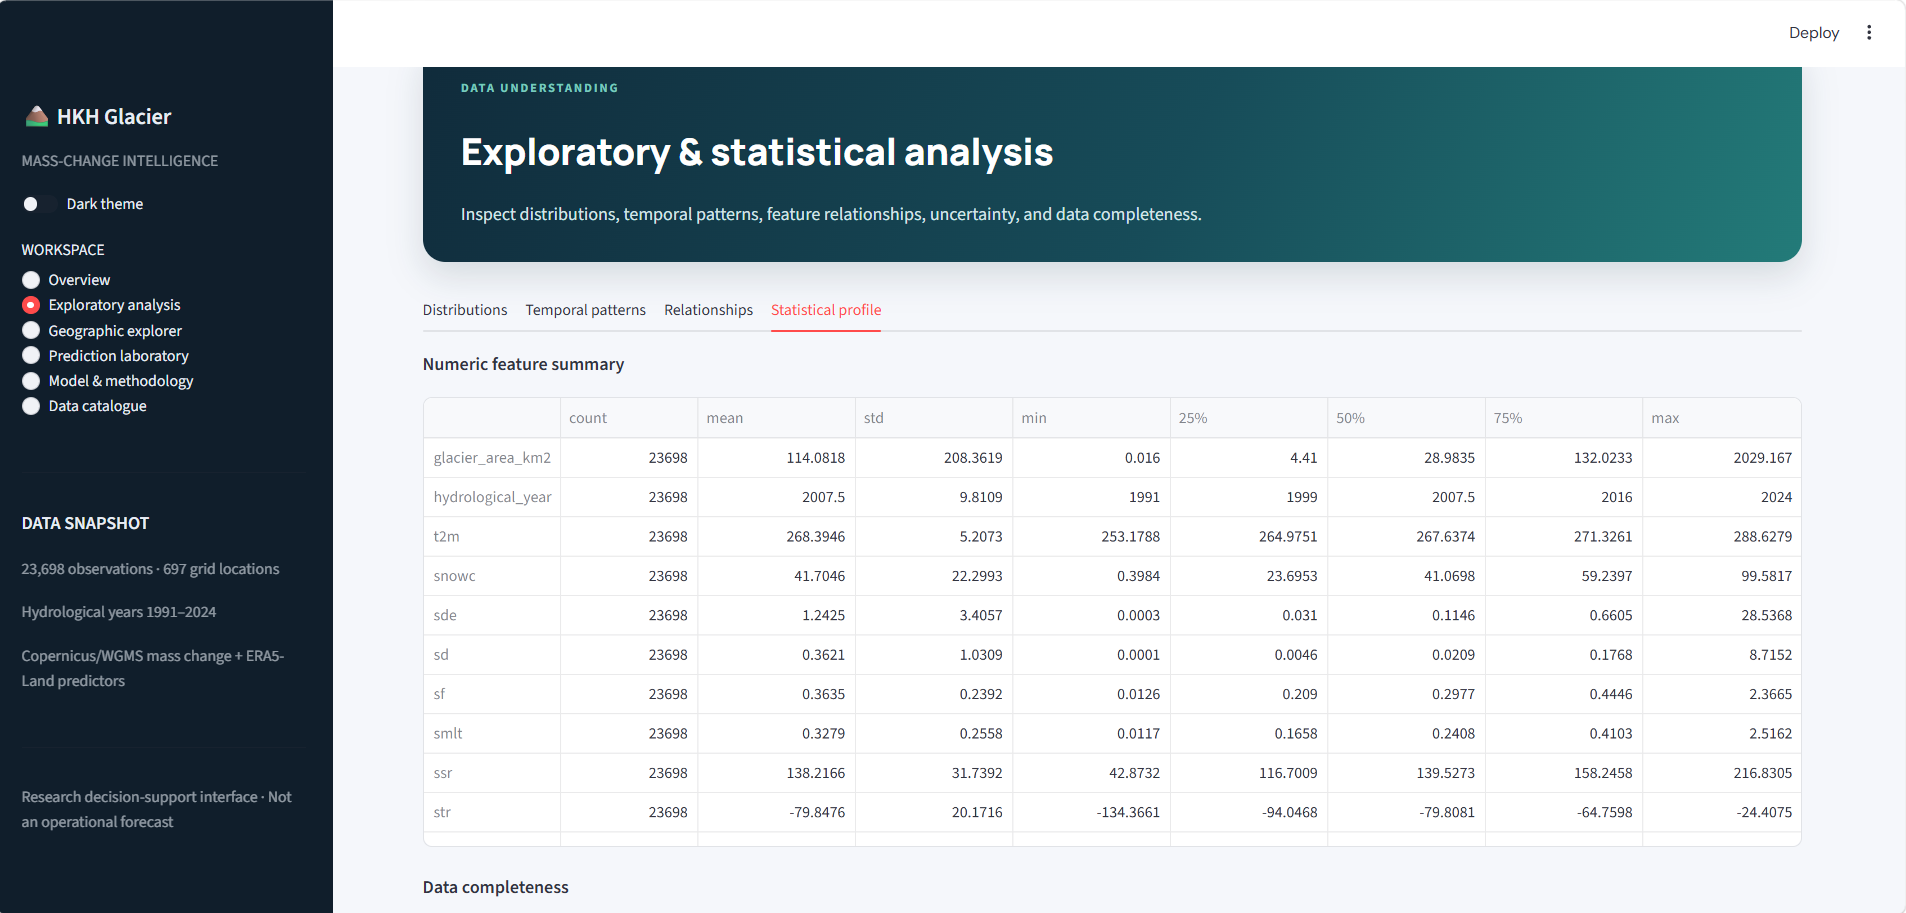
\includegraphics[width=\columnwidth]{dashboard_screenshots/exploratory_analysis_4.png}
\caption{Streamlit exploratory analysis: distributional diagnostic view.}
\label{fig:dashboard-exploratory-4}
\end{figure}

\begin{figure}[H]
\centering
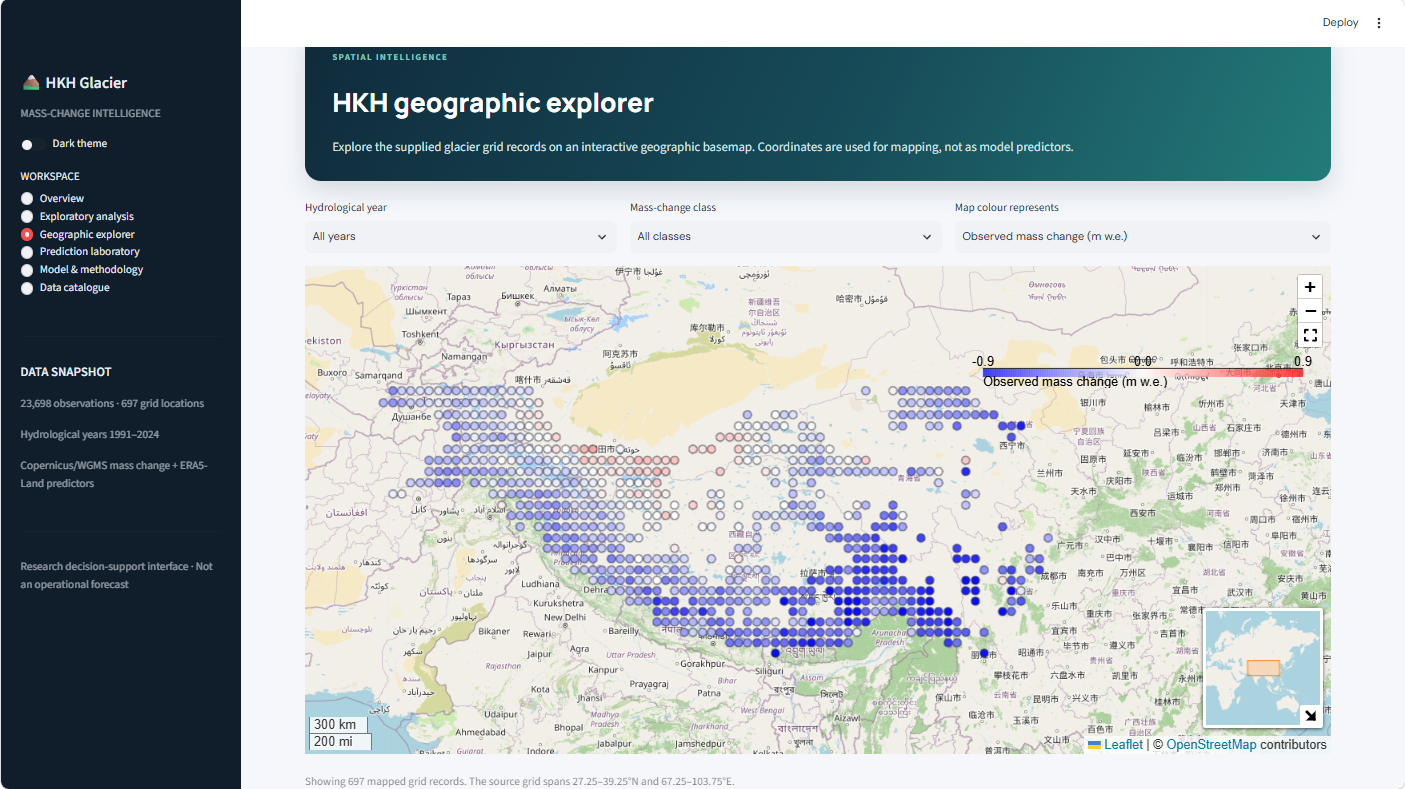
\includegraphics[width=\columnwidth]{dashboard_screenshots/geographic_explorer.png}
\caption{Streamlit geographic explorer.}
\label{fig:dashboard-geographic-explorer}
\end{figure}

\begin{figure}[H]
\centering
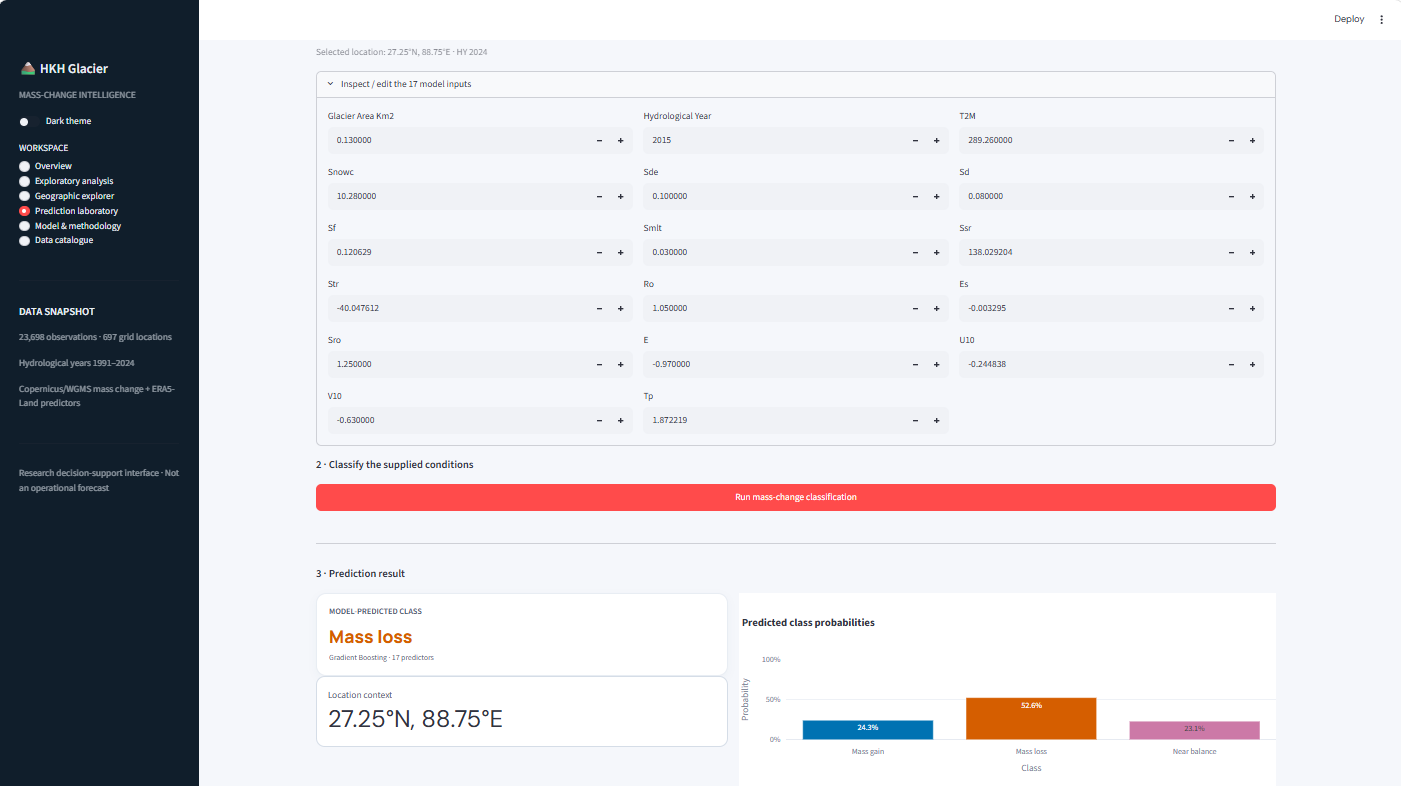
\includegraphics[width=\columnwidth]{dashboard_screenshots/prediction_laboratory_1.png}
\caption{Streamlit prediction laboratory: input controls and prediction interface.}
\label{fig:dashboard-prediction-laboratory-1}
\end{figure}

\begin{figure}[H]
\centering
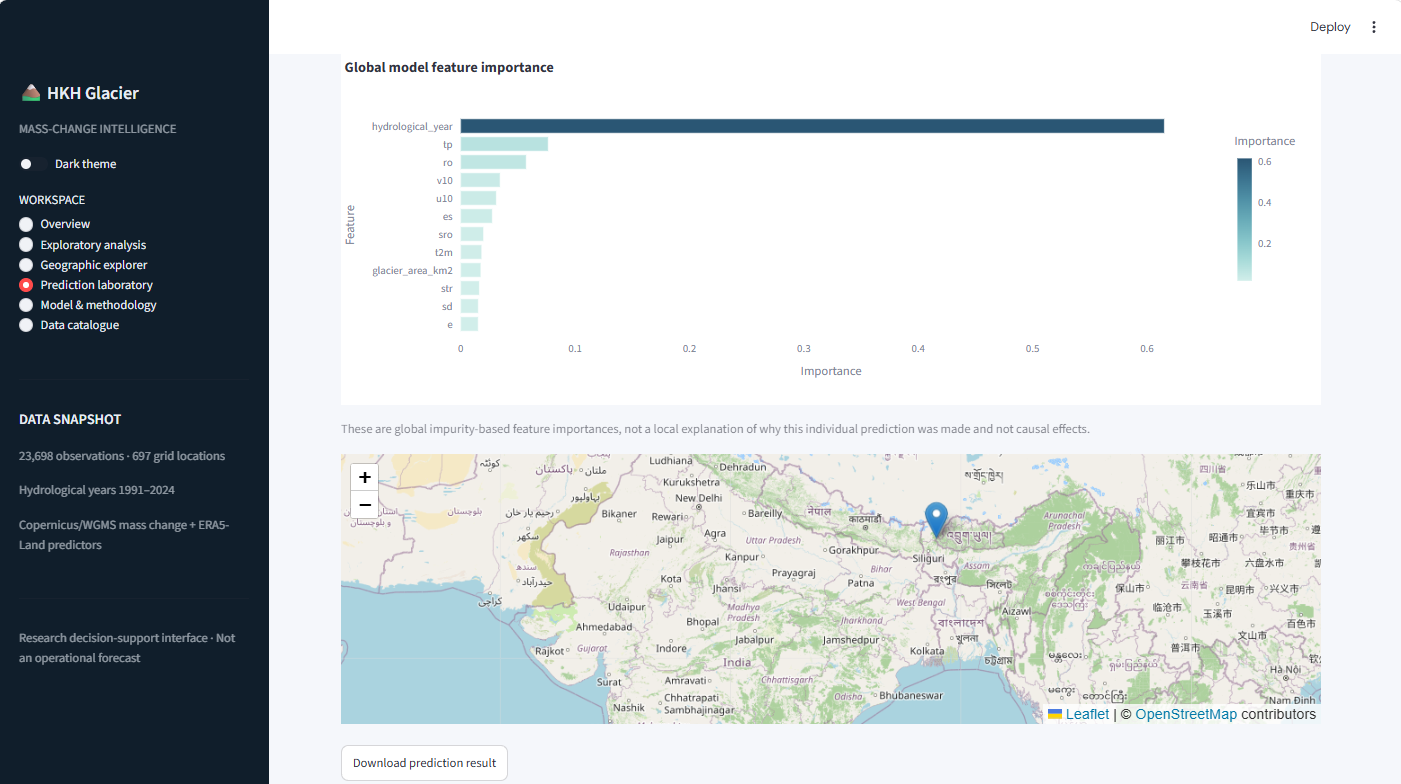
\includegraphics[width=\columnwidth]{dashboard_screenshots/prediction_laboratory_2.png}
\caption{Streamlit prediction laboratory: model output and probabilities.}
\label{fig:dashboard-prediction-laboratory-2}
\end{figure}

\begin{figure}[H]
\centering
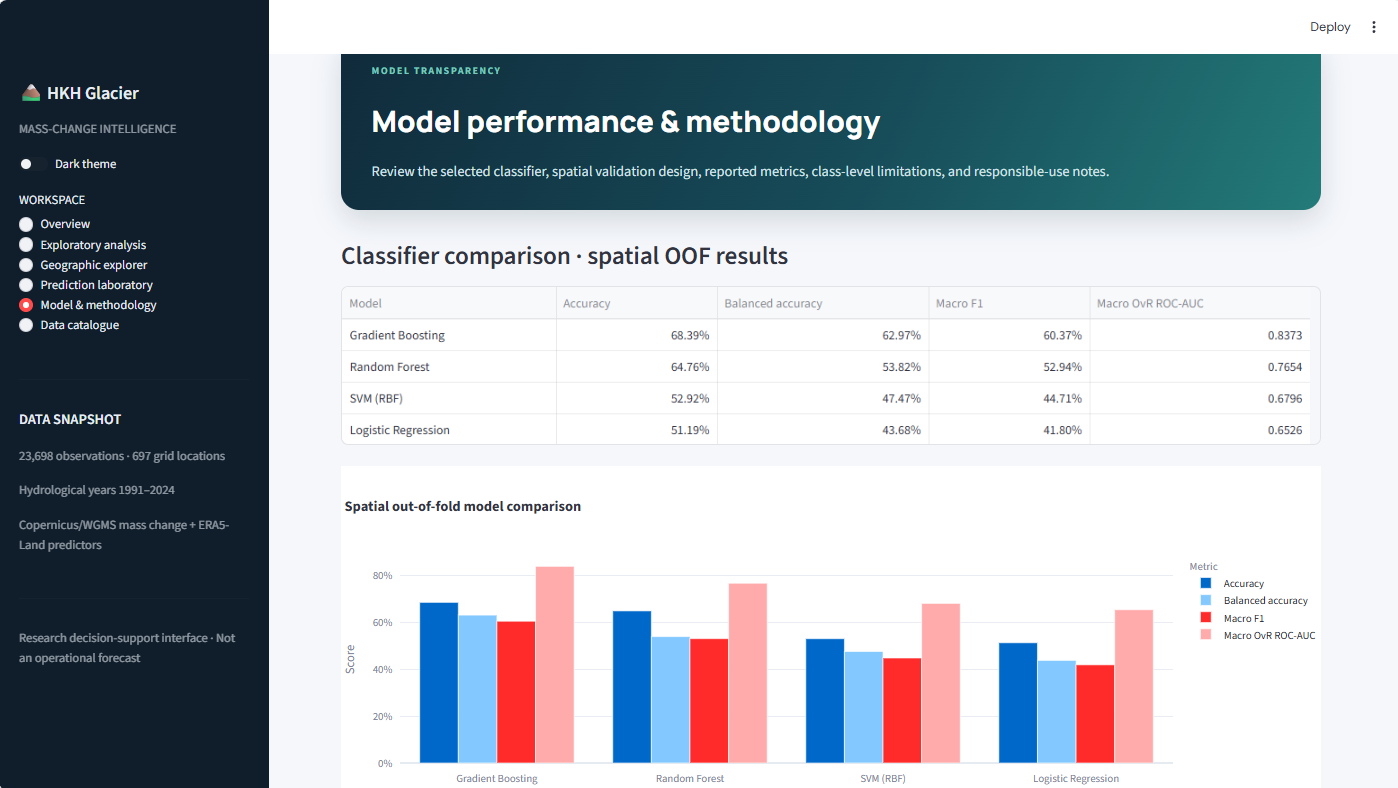
\includegraphics[width=\columnwidth]{dashboard_screenshots/model_methodology.png}
\caption{Streamlit model and methodology page.}
\label{fig:dashboard-model-methodology}
\end{figure}

\begin{figure}[H]
\centering
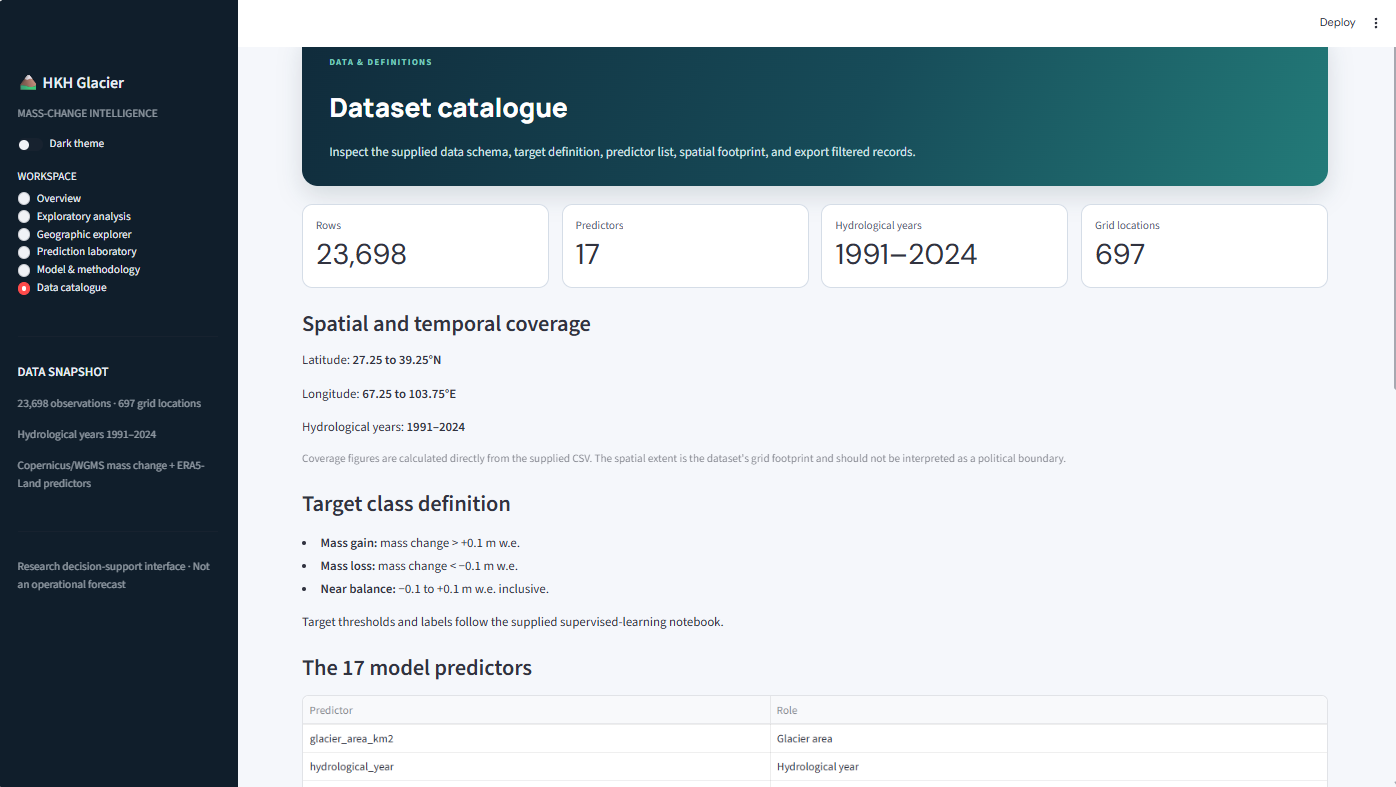
\includegraphics[width=\columnwidth]{dashboard_screenshots/data_catalogue.png}
\caption{Streamlit data catalogue page.}
\label{fig:dashboard-data-catalogue}
\end{figure}

\end{document}
